\documentclass[11pt,oneside]{book}
\usepackage{fontspec}
\usepackage{xeCJK}
\setmainfont{Latin Modern Roman}
\setCJKmainfont[ItalicFont={Noto Serif CJK JP},BoldItalicFont={Noto Serif CJK JP Bold}]{Noto Serif CJK JP}
\setCJKsansfont{Noto Sans CJK JP}
\setCJKmonofont{Noto Sans Mono CJK JP}
\newfontfamily\proseunicodefont{DejaVu Serif}
\usepackage[margin=1in]{geometry}
\usepackage{microtype}
\usepackage{amsmath,amssymb,amsthm,mathtools,bm}
\usepackage{graphicx}
\usepackage{xcolor}
\usepackage{booktabs}
\usepackage{array}
\usepackage{longtable}
\usepackage{enumitem}
\usepackage{float}
\usepackage{caption}
\usepackage{hyperref}
\usepackage{fancyhdr}
\usepackage{tikz}
\usetikzlibrary{arrows.meta,positioning,calc,decorations.pathmorphing}

\hypersetup{
  colorlinks=true,
  linkcolor=blue!50!black,
  urlcolor=blue!50!black,
  citecolor=blue!50!black
}

\setlength{\parskip}{0.5em}
\setlength{\parindent}{0pt}
\setlist[itemize]{topsep=0.25em,itemsep=0.2em}
\setlist[enumerate]{topsep=0.25em,itemsep=0.2em}
\setlength{\headheight}{40pt}
\numberwithin{equation}{chapter}

\newtheorem{theorem}{定理}[chapter]
\newtheorem{proposition}[theorem]{命題}
\newtheorem{lemma}[theorem]{補題}
\newtheorem{corollary}[theorem]{系}
\theoremstyle{definition}
\newtheorem{definition}[theorem]{定義}
\newtheorem{example}[theorem]{例}
\theoremstyle{remark}
\newtheorem{remark}[theorem]{注意}

\providecommand{\ket}[1]{\left\lvert#1\right\rangle}
\providecommand{\bra}[1]{\left\langle#1\right\rvert}
\providecommand{\braket}[2]{\left\langle#1\,\middle|\,#2\right\rangle}
\providecommand{\expect}[1]{\left\langle#1\right\rangle}
\newcommand{\lectureoverview}[1]{\paragraph{概観。} #1}

\makeatletter
\newcommand{\course@headerfont}{\normalfont\small\itshape}
\newcommand{\course@pagefont}{\normalfont\small}
\newcommand{\course@headerraise}{14pt}
\newlength{\course@headerboxheight}
\setlength{\course@headerboxheight}{\dimexpr\headheight-\course@headerraise-9pt\relax}
\newcommand{\course@leftheadbox}[1]{%
  \raisebox{\course@headerraise}{%
    \parbox[t][\course@headerboxheight][t]{0.82\textwidth}{%
      \raggedright\course@headerfont\strut\MakeUppercase{#1}\strut%
    }%
  }%
}
\newcommand{\course@rightheadbox}[1]{%
  \raisebox{\course@headerraise}{%
    \parbox[t][\course@headerboxheight][t]{0.82\textwidth}{%
      \raggedleft\course@headerfont\strut\MakeUppercase{#1}\strut%
    }%
  }%
}
\renewcommand{\chaptermark}[1]{\markboth{\MakeUppercase{\chaptername\ \thechapter.\ #1}}{}}
\renewcommand{\sectionmark}[1]{\markright{\MakeUppercase{\thesection\hspace{0.4em}#1}}}
\fancyhf{}
\fancyhead[L]{\course@leftheadbox{\leftmark}}
\fancyhead[R]{\course@pagefont\thepage}
\renewcommand{\headrulewidth}{0.5pt}
\pagestyle{fancy}
\fancypagestyle{plain}{%
  \fancyhf{}
  \fancyhead[L]{\course@leftheadbox{\leftmark}}
  \fancyhead[R]{\course@pagefont\thepage}
  \renewcommand{\headrulewidth}{0.5pt}
}
\makeatother

% Video2Book editorial provenance macros
\newenvironment{classroomqa}{%
  \par\medskip\noindent\begin{minipage}{\linewidth}\small\hrule\medskip
}{%
  \medskip\hrule\end{minipage}\par\medskip
}
\newcommand{\audiencequestion}[1]{\noindent\textbf{受講者からの質問。} #1\par\smallskip}
\newcommand{\lecturerresponse}[1]{\noindent\textbf{回答。} #1\par}
\newcommand{\lecturetimestamp}[1]{\footnote{講義時刻： #1.}}
\newcommand{\lectureframe}[1]{\par\smallskip{\centering\footnotesize\itshape 講義映像： #1.\par}}
\newcommand{\editorialnote}[1]{\footnote{編集上の補足： #1}}

\renewcommand{\contentsname}{目次}
\renewcommand{\chaptername}{章}
\renewcommand{\figurename}{図}
\renewcommand{\tablename}{表}
\renewcommand{\proofname}{証明}
\renewcommand{\bibname}{参考文献}
\emergencystretch=2em
\pdfstringdefDisableCommands{\def\proseunicodefont{}}

\geometry{paperwidth=177.6mm,paperheight=252mm,left=16mm,right=16mm,
 top=18mm,bottom=18mm,includeheadfoot,headheight=28pt,headsep=7mm,footskip=9mm}
\usepackage{scrextend}
\changefontsizes[17pt]{12pt}
\raggedbottom
\renewenvironment{classroomqa}{\par\medskip\begingroup}{\par\endgroup\medskip}
\fancyhf{}
\setlength{\headwidth}{\textwidth}
\fancyhead[L]{\parbox{\textwidth}{\raggedright\fontsize{9}{11}\selectfont\nouppercase{\leftmark}}}
\fancyfoot[C]{\small\thepage}
\renewcommand{\headrulewidth}{0.3pt}
\fancypagestyle{plain}{\fancyhf{}\fancyfoot[C]{\small\thepage}\renewcommand{\headrulewidth}{0pt}}

\graphicspath{{../../../generated_course_notes/core/cosmology/2009_winter_legacy_cosmology/figures/}{../../../generated_course_notes/core/cosmology/2009_winter_legacy_cosmology/assets/}}
\begin{document}
\frontmatter
\hypersetup{pageanchor=false}
\begin{titlepage}
\thispagestyle{empty}
\begin{tikzpicture}[remember picture,overlay]
  \node[anchor=center,inner sep=0] at (current page.center) {%
    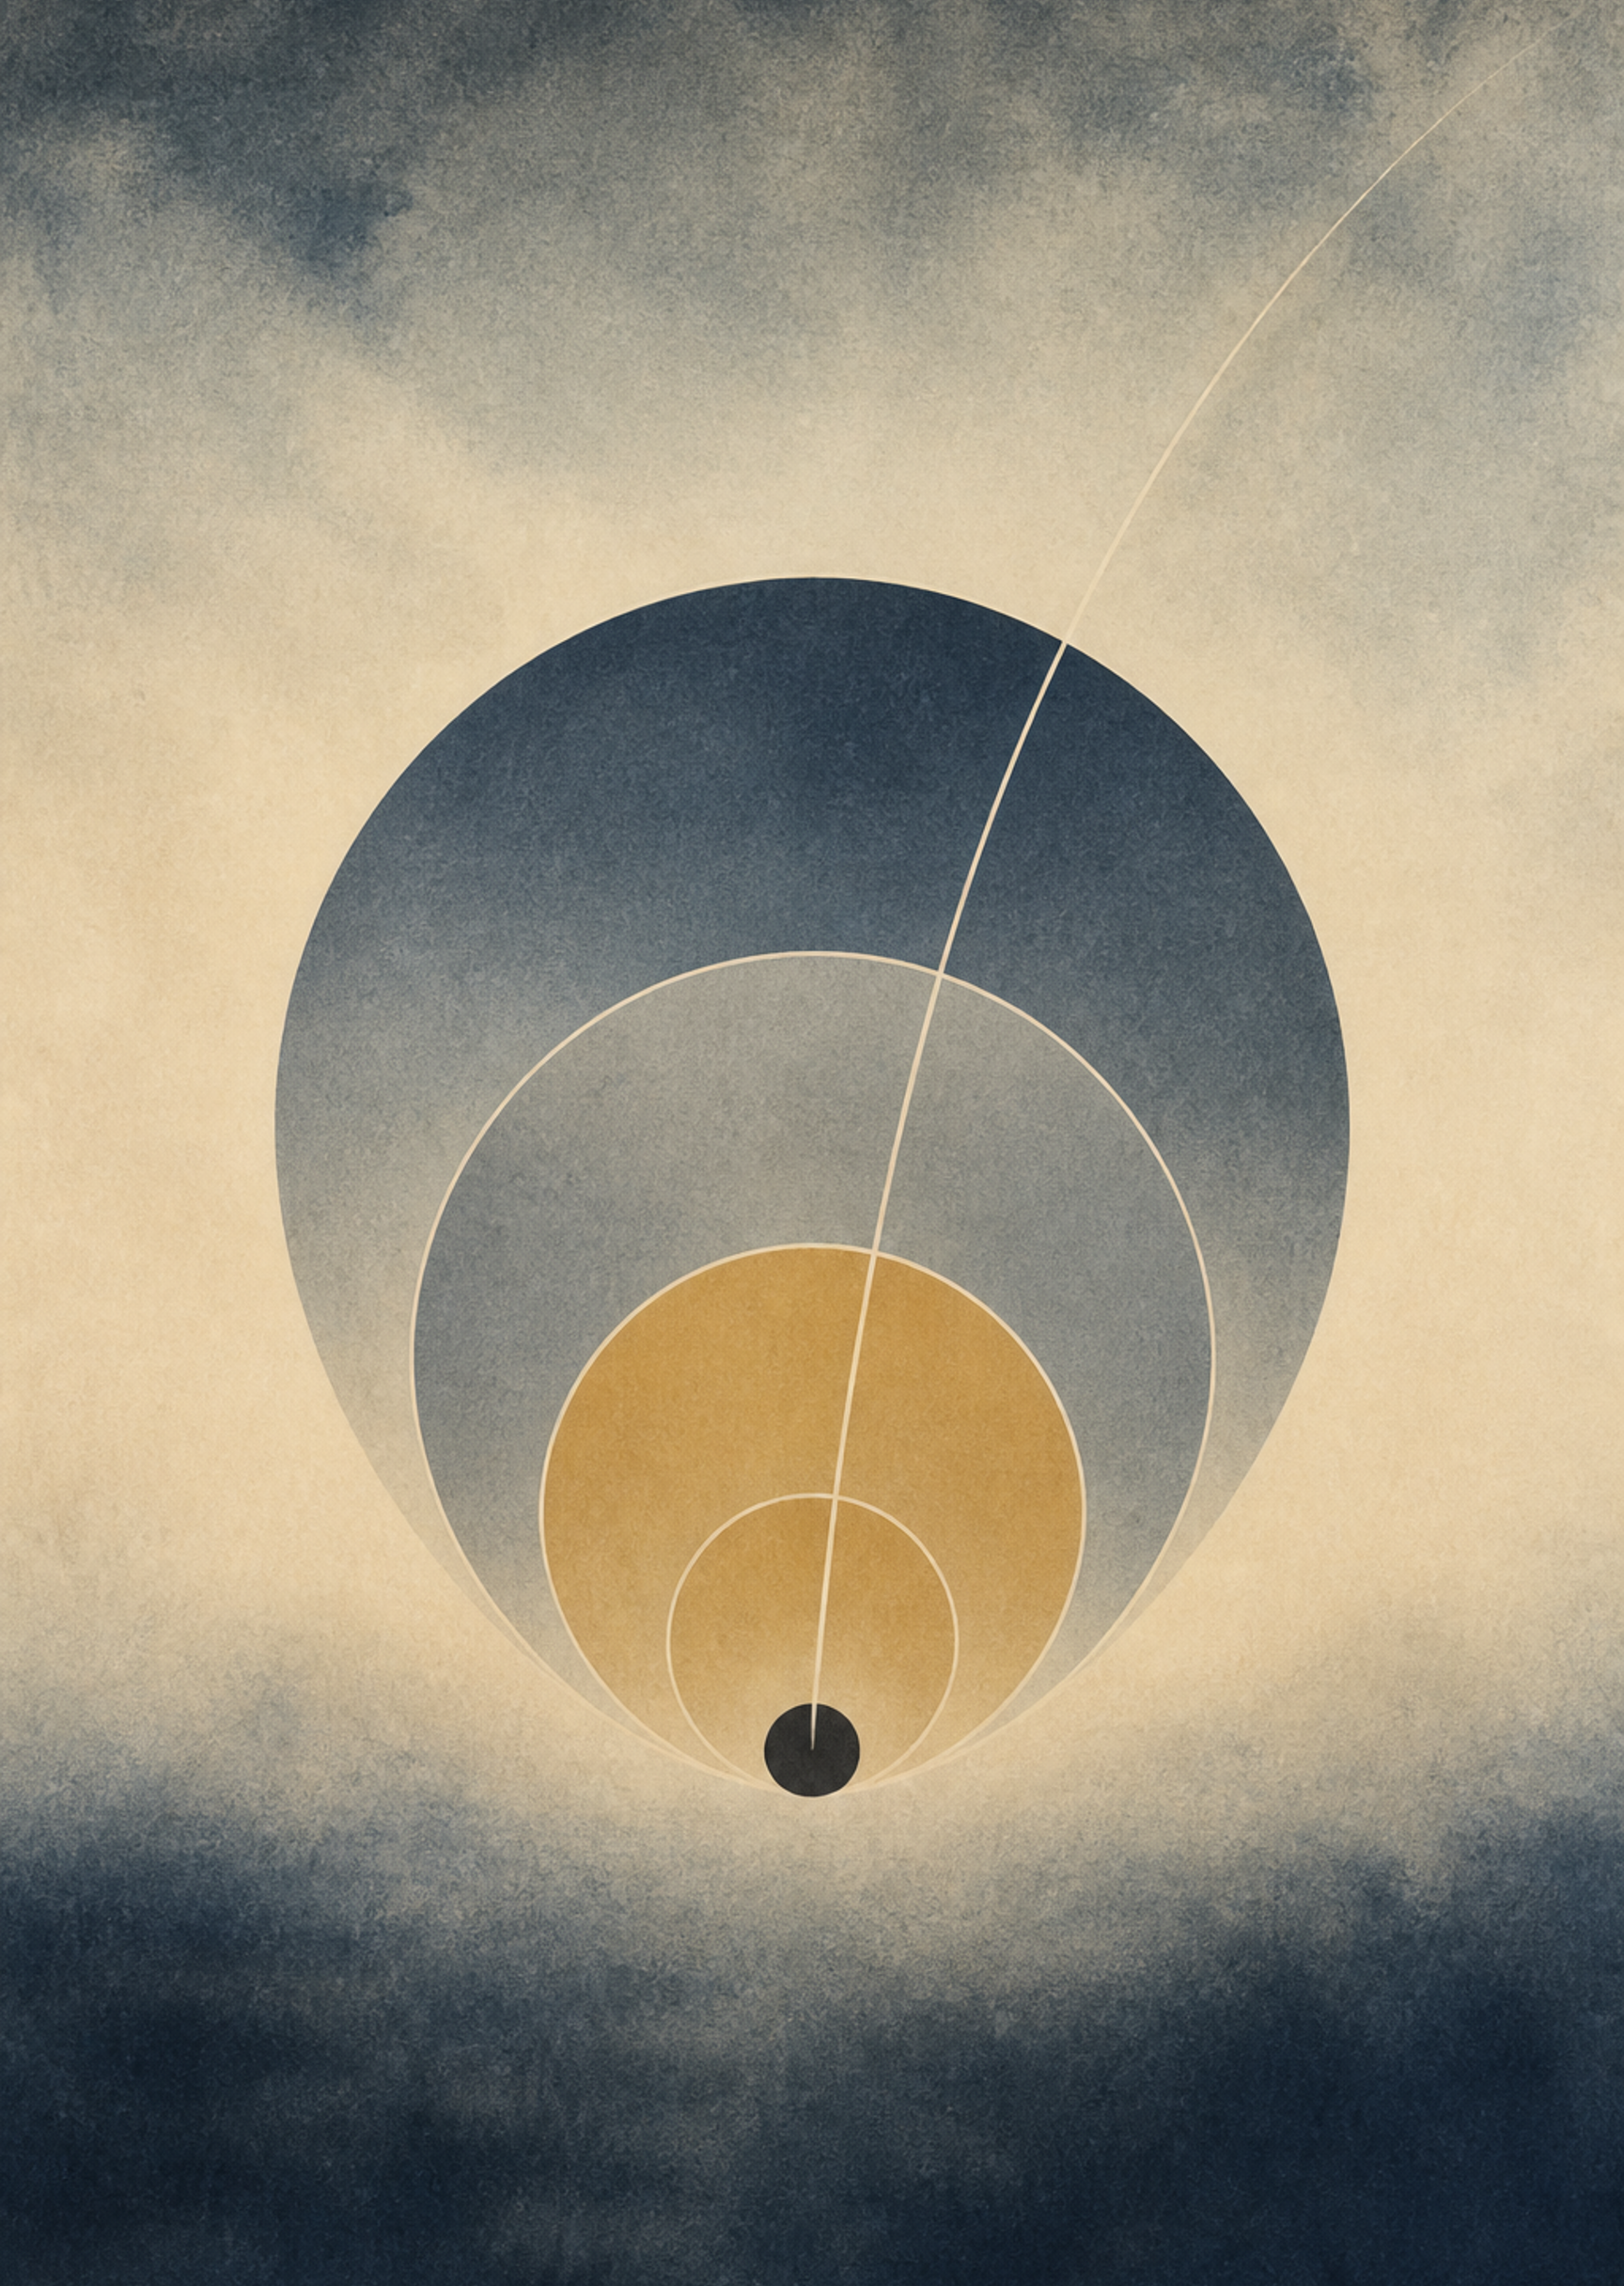
\includegraphics[height=\paperheight,keepaspectratio]{../../../generated_course_notes/core/cosmology/2009_winter_legacy_cosmology/assets/cover-art.png}%
  };
  \node[
    anchor=north west,
    align=left,
    text width=0.78\paperwidth,
    fill=white,
    fill opacity=0.9,
    rounded corners=8pt,
    inner xsep=10pt,
    inner ysep=8pt
  ] at ([xshift=0.08\paperwidth,yshift=-0.06\paperheight]current page.north west) {%
    {\fontsize{30}{33}\selectfont\bfseries\color{black!88} 宇宙論\\[0.85em]}
    {\large\color{black!72} 日本語版 / 2009 winter legacy cosmology}
  };
  \node[
    anchor=south west,
    align=left,
    text width=0.68\paperwidth,
    fill=white,
    fill opacity=0.82,
    text opacity=1,
    rounded corners=6pt,
    inner sep=12pt
  ] at ([xshift=0.08\paperwidth,yshift=0.08\paperheight]current page.south west) {%
    {\normalsize\color{black!78} 原講義：Leonard Susskind\\[0.35em]}
    {\small\color{black!72} 講義補助版：\href{https://lazying.art}{LazyingArt LLC} / \href{https://github.com/lachlanchen/Video2Book}{Video2Book}}
  };
\end{tikzpicture}
\mbox{}
\end{titlepage}
\hypersetup{pageanchor=true}

\clearpage
\chapter*{このノートについて}
これらの独立に編集された伴走ノートは、レナード・サスキンドによる講義に基づくものである。これらは機械文字起こし、字幕、および選択された黒板のフレームから再構成され、その後、利用可能な原資料と照合された。これらはサスキンド教授による原著原稿ではなく、同教授による査読や承認も受けていない。

本版は\href{https://lazying.art}{LazyingArt LLC}がオープンソースの\href{https://github.com/lachlanchen/Video2Book}{Video2Book}ワークフローを用いて作成した。機械文字起こしは別途利用可能であり、認識誤りを含む可能性がある。編集上の明確化および自明でない再構成は脚注で示されている。
\clearpage
\tableofcontents
\mainmatter
\chapter{膨張宇宙の幾何学}

要点は膨張宇宙とその幾何学である。目的は、膨張を駆動するものを問う前に、空間が膨張するとはどういうことかを記述することである。ニュートン的な\(F=ma\)宇宙論は後で扱い、その後に初めて幾何学と力学が完全なフリードマン--ロバートソン--ウォーカー枠組みへと組み立てられる。

\section{膨張する直線上の共動座標}

最も単純な例から始めよう。時空ではなく一次元空間である。等間隔に銀河が並んだ無限の直線を想像する。座標\(x\)はまだ物理的な距離を測ってはいない。それは銀河にラベルを付けるものである。\(x\)を銀河の名前と考えることができ、その名前は、配置全体が伸び縮みしても銀河に付いたままである。

\(x=0\)と呼ばれる銀河から\(x=1\)と呼ばれる銀河までの物理的距離を\(a\)とする。すると任意の二つの銀河の間の物理的距離は
\begin{equation}
d=a\,\Delta x.
\end{equation}
である。座標差\(\Delta x\)は単にラベルの差にすぎない。因子\(a\)がそのラベル差を、物差しで測られる実際の距離に変換する。

次に、この直線を伸びる弾性糸として想像しよう。ラベルは銀河に付いたままであるが、隣り合う銀河の間の距離は時間とともに変化する。同じ関係は
\begin{equation}
d(t)=a(t)\,\Delta x.
\end{equation}
となる。この段階で、一様性とは単に、隣り合う銀河がどこでも等間隔に並んでいることを意味する。ただしその共通の間隔は時間とともに変化しうる。

\section{ハッブルの法則と中心の不在}

二つの固定された銀河の相対速度を求めるには、その対を固定して\(\Delta x\)が時間とともに変化しないようにする。微分すると
\begin{align}
\dot d &= \dot a\,\Delta x \\
       &= \frac{\dot a}{a}\,a\,\Delta x \\
       &= \frac{\dot a}{a}\,d.
\end{align}
が得られる。ここで
\begin{equation}
H(t)\equiv \frac{\dot a}{a},
\end{equation}
と定義すれば、
\begin{equation}
\dot d = H(t)\,d.
\end{equation}
となる。これがハッブルの法則である。

歴史的な表現である``ハッブル定数''は誤解を招く。この量は時間的にではなく空間的に一定である。ある瞬間にはどの銀河に対しても同じであるが、一般には宇宙の進化とともに変化する。ハッブルパラメータと考えた方がよい。

この法則は、より遠い銀河ほど速く後退することを述べている。それは中心を特別扱いしない。この議論のどこにも\(x=0\)やその他の点を特権化するものはない。どの観測者も同じ規則を見る。したがってこの模型における膨張宇宙は、一つの特別な場所からの爆発ではない。

赤方偏移は直ちに現れる。二つの銀河が互いに離れながら光信号を交換すると、受け取る光は赤くなる。後退速度が大きいほど赤方偏移も大きい。したがってスペクトル線は後退速度について教えてくれる。距離の測定はより難しく、ハッブルの初期の推定は粗かった。彼の最初のプロットは完全な直線ではなく、大きな不確かさをもつ散らばった点の集合であった。それでも、幾何学的原理はノイズを生き延びた。後退速度は距離に比例するのである。

\begin{classroomqa}
\audiencequestion{銀河が十分に離れていれば、ハッブルの法則によってそれらは光速より速く動くのか。}\lecturetimestamp{00:20:23}
\lecturerresponse{はい、この後退の意味ではそうなる。君の言っていることは正しい。それについては必ず後で戻ってくる。それは最も重要な事柄の一つである。}
\end{classroomqa}

\section{高次元、等方性、そして\(a(t)\)の時間依存性}

空間次元が増えても本質的なことは何も変わらない。二次元では\((x,y)\)でラベル付けされた銀河の正方形格子を、三次元では\((x,y,z)\)でラベル付けされた銀河の格子を想像する。座標は再び共動ラベルである。それらは物理的距離を直接測るのではなく、銀河とともに動く。

\(x\)方向の間隔が\(y\)方向の間隔と同じであるべきなのはなぜか。答えは観測による。もし銀河がある方向で別の方向より系統的に密集していれば、空は方向によって異なって見えるだろう。十分に大きなスケールではそうはならない。この方向に関する同一性が等方性である。

二次元では二つの銀河の間の距離は
\begin{equation}
d=a\sqrt{(\Delta x)^2+(\Delta y)^2},
\end{equation}
であり、三次元では
\begin{equation}
d=a\sqrt{(\Delta x)^2+(\Delta y)^2+(\Delta z)^2}.
\end{equation}
である。固定された銀河の対に対して座標差は一定に保たれるので、再び微分すると
\begin{equation}
\dot d=\frac{\dot a}{a}\,d.
\end{equation}
が得られる。ハッブルの法則は変わらない。

一様性とは場所から場所への同一性を意味する。等方性とは方向から方向への同一性を意味する。どちらも小さなスケールでは厳密ではない。天の川を通して見ることはその平面の外を見ることとは異なり、個々の銀河は短い距離では一様に分布していない。しかし多くの銀河について平均すれば、大きなスケールの宇宙はどこでも、どの方向でもほぼ同じに見える。

\begin{classroomqa}
\audiencequestion{速度が距離に比例し、距離が増大しているなら、固定された銀河の一対は互いに加速しながら遠ざかっていなければならないのだろうか。}\lecturetimestamp{00:40:22}
\lecturerresponse{いいえ。ハッブルの法則が述べているのは、ある瞬間において後退速度が距離に比例するということである。それ自体は、固定された一対の速度が時間とともに増大するか減少するかについては何も述べていない。それは\(a(t)\)の詳細な時間依存性に依存する。\(a(t)\propto t\)ならば、隣り合う銀河は一定の速さで離れていく。\(a(t)\propto t^2\)ならば、固定された一対の後退速度は時間とともに増大する。\(a(t)\propto \log t\)ならば、それは時間とともに減少する。法則\(\dot d=(\dot a/a)d\)は距離の関数として常に成り立つが、加速と減速は別個の問題である。}
\end{classroomqa}

長い間、宇宙論研究者たちは宇宙は減速していると予想していた。重力は、投げ上げられた物体を減速させるのと同じように、初期の膨張を遅くするはずだからである。ここでの要点はただ、ハッブルの法則だけでは\(\dot a\)や\(\ddot a\)の振る舞いは決まらないということである。

\begin{classroomqa}
\audiencequestion{スケール因子\(a\)の初期値はどのように設定するのですか。}\lecturetimestamp{00:46:18}
\lecturerresponse{その全体的な規格化は任意である。物理的に重要なのは、\(a\)の数値的な大きさそのものではなく、それがどのように変化するかである。別のスケール因子\(b=3a\)を定義すると、\(\dot b/b=\dot a/a\)となる。\(a\)を定数で再スケールすることは、慣習や単位を変えるだけであって、ハッブルパラメータを変えるものではない。}
\end{classroomqa}

\section{空間計量から時空計量へ}

ここで\(\Delta x\)を\(dx\)に置き換える。隣り合う点の間の物理的距離は
\begin{equation}
ds=a\,dx,
\end{equation}
であるから
\begin{equation}
ds^2=a^2\,dx^2.
\end{equation}
これが一次元における空間計量である。\(dx^2\)の係数は
\begin{equation}
g_{xx}=a^2.
\end{equation}
したがって、膨張する宇宙は、計量の空間部分が時間に依存すると言うことによって記述できる。

空間から時空へ移るには、相対論的間隔を用いる。一次元の空間では、
\begin{equation}
d\tau^2=dt^2-a^2(t)\,dx^2.
\end{equation}
共動観測者に対しては\(dx=0\)であるから、\(d\tau=dt\)となる。通常の宇宙時間とは、銀河とともに動く時計によって測られる固有時である。

この時点での黒板の図は、共動世界線、線素、計量の記法をまとめて示すので有用である。
\begin{figure}[H]
\centering
\includegraphics[width=0.82\textwidth]{lecture_01_figure_02.png}
\caption{膨張する一次元宇宙における共動世界線と、対応する時空間隔。}
\end{figure}

三次元の空間では、同じパターンから慎重な拡張が得られる\footnote{黒板は00:56:38--00:58:51のあたりで一部が隠れている。この三次元の形は、一次元の空間から三次元への口頭での拡張と、黒板上で見える対角パターンに従っている。}
\begin{equation}
d\tau^2=dt^2-a^2(t)\bigl(dx^2+dy^2+dz^2\bigr),
\end{equation}
対角計量
\begin{equation}
g_{\mu\nu}=\mathrm{diag}\bigl(1,-a^2,-a^2,-a^2\bigr).
\end{equation}
非対角項は消える。
\begin{equation}
g_{tx}=g_{ty}=g_{tz}=0.
\end{equation}

一様性とは、計量の係数が時間には依存してもよいが空間位置には依存しないことを意味する。等方性とは、三つの空間方向が同じように入ることを意味する。

\begin{classroomqa}
\audiencequestion{\(dx\)を距離と考えるべきではないのですか。}\lecturetimestamp{01:01:18}
\lecturerresponse{いいえ。\(dx\)は距離ではない。\(a\,dx\)が距離である。\(dx\)は単なるラベル間隔である。これを考えるのに有用なのは、ある瞬間に誰かが銀河を通る座標の網を描き、その網が銀河に従うことを要求すると想像することである。座標の間隔は構成上固定されたままだが、物理的距離は変化する。距離の単位を\(a\)ではなく\(x\)に入れることもできる。それは慣習である。重要なのは積\(a\,dx\)である。}
\end{classroomqa}

\begin{classroomqa}
\audiencequestion{\(dt^2\)の計量係数が\(1\)に等しいのは、これも単に慣習によるのですか。}\lecturetimestamp{01:03:24}
\lecturerresponse{はい。それ自体には物理はない。係数が時間だけに依存するなら、時間変数を変えてそれがちょうど\(dt^2\)になるようにできる。同様に\(c=1\)とする単位を選んでもよい。ここで慣習でないのは、係数が位置に依存しないことである。ただし時間には依存してもよい。}
\end{classroomqa}

\begin{classroomqa}
\audiencequestion{これをアインシュタインの場の方程式に入れると、エネルギー運動量テンソルについて何が得られますか。}\lecturetimestamp{01:05:59}
\lecturerresponse{それは次に来る種類の問いであるが、動力学に属するものであって、現在の議論には属さない。この計量をアインシュタイン方程式に入れて、どのようなエネルギー運動量分布がそれを解にするかを問うことができる。それは非常に重要であるが、当面の主題は動力学ではなく幾何学である。}
\end{classroomqa}

\section{地平線が隠すもの}

大規模な宇宙が一様かつ等方であるとみなされるのは、あくまで近似としてである。恒星、惑星、あるいは個々の銀河のスケールでは、決して一様ではない。あらゆる局所的な観測において厳密に等方であるわけでもない。

農家の畑は、正しいスケール依存性を与えてくれる。あるスケールでは規則的に見えるが、はるかに小さいスケールでは明らかにそうではない。畑全体より大きいスケールでは、再び一様には見えなくなる。宇宙論も同じように成り立つ。多数の銀河について平均すれば、大規模な分布はほぼ一様に見える。十分に小さいスケールではそうではない。

宇宙は、われわれが見ることのできる部分より大きく、またわれわれが決して見ることのできない部分よりも大きい。実際に探ることのできるスケールでは、局所的な変動を別にすれば、等方かつ一様である。それを超えると、直接的な観測的保証は何もない。

\begin{classroomqa}
\audiencequestion{われわれは決して直接には突き止められないだろうとおっしゃいました。それは、間接的に突き止める方法があり得るという意味でしょうか。}\lecturetimestamp{01:10:34}
\lecturerresponse{おそらく。近ごろの大方の考えでは、十分に大きなスケールでは宇宙は一様ではない。私自身の賭けも同じである。しかしそれは、私が決して勝つことも負けることもない賭けだ。基本的な理由により、われわれは現在見えるところよりずっと遠くを見ることはできないからである。すなわち、地平線の存在である。}
\end{classroomqa}

\begin{classroomqa}
\audiencequestion{見える範囲を超えた質量を探すのに、重力を利用することはできないのでしょうか。}\lecturetimestamp{01:11:53}
\lecturerresponse{できない。遠方の質量は、われわれを単に自由落下させることができるだけである。閉じた部屋に座っていても、われわれは太陽の重力場の中にあり、その周りを公転しているが、外を見なければ、太陽がそこにあると簡単に見分ける方法はない。それを明らかにするのは潮汐力だけであり、源が十分に遠ければ、その潮汐効果は検出できないほど小さくなりうる。}
\end{classroomqa}

したがって地平線は、直接的な知識への究極の障壁である。彼はさらに、ほぼ確実に、宇宙はわれわれが決して見ることのできない領域よりも体積で少なくとも千倍大きいと述べ、その主張の根拠は後回しにしている。

\section{境界はあるが端はない}

次に閉じた幾何学に移る。無限直線は開いており、非有界である。線分は、有限の広がりしか持たないという意味で有界である。有界とは境界があるという意味ではなく、有限の広がりを持つという意味である。

壁のある立方体ではうまくいかない。それは一様性を破る。壁の近くにいる者と壁から遠くにいる者は等価ではないからである。また等方性も破る。中心にいる者でさえ、方向によって異なるものを見るからである。

円や球の内部も同様に失敗する。中心にいる者はどの方向にも同じものを見るが、その対称性はただ一つの特別な点に属するだけである。中心から離れれば、壁はある方向には近く、別の方向には遠い。するとその空間は、一般的な観測者にとって一様でも等方でもない。

非常に大きなスケールでは、宇宙は一様かつ等方であるというのが作業仮説である。これが宇宙原理である。それは有用だが、改訂から守られてはいない。

\begin{classroomqa}
\audiencequestion{至る所で等方であることは、一様であることを含意するのでしょうか。}\lecturetimestamp{01:18:57}
\lecturerresponse{はい。すべての観測者がどの方向にも同じものを見るならば、それは一様性を含意する。しかし逆は成り立たない。一様性それ自体は等方性を含意しない。宇宙は一様でありながら、なお優先方向を持つことができる。たとえば、すべて同じ向きを指す矢で満たされていればそうである。}
\end{classroomqa}

正しい有界模型は、特徴のない球の表面である。その表面に閉じ込められた二次元の生物は、世界が有限であっても、あらゆる場所が局所的に他のあらゆる場所と同じであり、あらゆる方向が他のあらゆる方向と同じであると見いだす。これが、端のない境界である。

\section{円上の閉じた一次元宇宙}

代数を簡単に保つため、球の例を一次元の空間、すなわち円上の生活に還元する。一次元では、等方性とは左と右が等価であることを意味する。円はまさにその特徴を持つ。一点を選び、それを\(\theta=0\)と呼ぶ。他のすべての点は、ラジアンで測られる角度座標\(\theta\)によってラベル付けされる。原点の一方の側すぐの点は、小さな負の角度によっても、\(2\pi\)のすぐ手前の角度によっても記述できる。この周期性は幾何学の一部である。

円の住人は、外部の半径や中心ではなく、円周にアクセスできる。彼らは、同じ点に戻るまで円に沿って進むことによって、周囲の全距離を測ることができる。周囲の平面に円を描くならば、半径に似た量を導入してもよいが、それは埋め込みの描像に属するものであり、彼らが測る内在的な幾何学に属するものではない。

ここでは黒板の図が役に立つ。角度のラベルと全周長を同じ図に保つことができるからである。
\begin{figure}[H]
\centering
\includegraphics[width=0.82\textwidth]{lecture_01_figure_03.png}
\caption{全周長\(2\pi a\)の閉じた一次元宇宙の角度による記述。}
\end{figure}

便利な慣習は\footnote{01:26:40--01:29:20頃、記法は全円周そのものをスケール因子とみなす場合と、それを\(2\pi a\)と書く場合との間で一時的に揺れる。ここでは後者の慣習を用いる。それは弧長の公式に引き継がれる慣習だからである。}
\begin{equation}
L=2\pi a,
\end{equation}
ここで\(L\)は全円周である。

小さな角度差\(\Delta\theta\)に対して、物理的距離は
\begin{equation}
d=a\,\Delta\theta.
\end{equation}
である。無限小に移行すると
\begin{equation}
ds=a\,d\theta,
\end{equation}
となり、したがって
\begin{equation}
ds^2=a^2\,d\theta^2.
\end{equation}
である。これが円上の局所計量である。

\(a\)が時間に依存するなら、閉じた一次元宇宙は膨張または収縮する。固定された一対の銀河に対して、
\begin{equation}
d(t)=a(t)\,\Delta\theta,
\end{equation}
であるから、
\begin{equation}
\dot d=\dot a\,\Delta\theta
      =\frac{\dot a}{a}\,d.
\end{equation}
となる。ここでもハッブルの法則は生き残る。少なくとも、円の反対回りが曖昧になるほど離れていない一対に対しては。

時空計量は
\begin{equation}
d\tau^2=dt^2-a^2(t)\,d\theta^2.
\end{equation}
となる。\(a\)が一定なら、時空の描像は円柱である。\(a\propto t\)なら、それは円錐である。\(a(t)\)がより不規則に変化するなら、描像は花瓶のようになる。

この描像を逆向きにたどると、銀河はどんどん近づいていく。円の周りに\(360\)個の銀河があったなら、遅い時刻にはよく広がっており、より早い時期には非常に近く集まり、さらに早くにはもっと近くなる。やがてそれらはもはや別々の銀河ではなくなり、さらに早くには別々の原子ですらなくなる。しかしそれでも、空間に特別な点は存在しない。

これが、この模型においてビッグバンがどこで起こったかという問いへの最も明快な答えである。\(a(t)\to 0\)となると、すべての間隔\(a(t)\,\Delta\theta\)はゼロに向かう。宇宙全体が至る所で同時に縮む。銀河は外部空間の特権的な位置から飛び去っているのではない。幾何学そのもののスケールが変化している。その意味で答えは、至る所である。

\begin{classroomqa}
\audiencequestion{時空は曲がっていると言いました。それが円柱だったとしても曲がっているのですか。}\lecturetimestamp{01:38:04}
\lecturerresponse{いいえ。もしそれが円柱なら、曲がってはいない。それは\(a\)が時間的に一定である場合である。曲がって見えるのは、より高次元の空間に描かれているからにすぎない。それを切り開けば、引き伸ばすことなく平らに広げられる。}
\end{classroomqa}

そこから議論は円錐へ移る。\(a\propto t\)なら、時空の描像は円錐である。その先端から離れたところでは、円錐も同じ内在的な意味で平らである。すなわち、平面に開くことができる。先端は異なる。それは円錐特異点である。

次の段階は、球状宇宙の幾何学、そして\(a(t)\)がどのように成長または縮小するかを決める力学である。

\chapter{ニュートン宇宙論とフリードマン方程式}

前回は空間の計量について話した。次の問題は力学である。スケール因子は時間とともにどのように変化するのか。まず少し幾何学から始め、それからニュートン宇宙論に進む。フリードマン方程式はまだ一般相対性理論から導出されない。それはニュートンの方程式から導出される。

\section{一様性、等方性、そして時間依存の計量}

一様性と等方性は前提として置かれている。宇宙が一様かつ等方であり、時間とともに変化するならば、ハッブルの法則は常に成り立つ。任意の固定された時刻において、後退速度は距離に比例する。
\begin{equation}
v = H(t)\,d.
\end{equation}
比例関係は線形である。一定なのは時間ではなく空間である。同じ比例係数が、与えられた瞬間のどこでも当てはまる。

\begin{classroomqa}
\audiencequestion{それは線形に比例するという意味ですか。}\lecturetimestamp{00:02:06}
\lecturerresponse{はい。固定された時刻において、後退速度は距離に線形に比例する。比例係数はハッブル定数である。一般にはそれは時間に依存するが、空間の点ごとに変わることはない。}
\end{classroomqa}

だからこそ「``ハッブル定数''」という表現は危険である。それは空間内の位置に対して一定である。時間に対して一定ではない。

次に自然な疑問が生じる。空間が膨張するなら、なぜ物差しも膨張しないのか。答えは、物差しは原子スケールにおける宇宙論的膨張に伴ういかなるものよりもはるかに強い力によって結合されているということである。束縛された物体は束縛されたままでいる。膨張するのは、十分に切り離されたものの間の距離である。例えば、互いを強く結びつけておくには離れすぎている銀河のようなものである。

\begin{classroomqa}
\audiencequestion{測定棒も膨張しているという事実について何か問題がありますか。}\lecturetimestamp{00:04:00}
\lecturerresponse{いいえ。測定棒は膨張していない。座標が膨張している。物差しを結合している力は、膨張による効果よりもはるかに強いので、通常の束縛された物体は背景とともに膨張しない。十分に離れた銀河は確かに離れていくが、物差しは膨張しない。}
\end{classroomqa}

原子間に微小な余分の斥力効果を想像することもできる。それでも棒を引き裂くことはない。それは、小さな余分の引力が硬いばねの平衡位置を変えるのと同じように、平衡間隔をほんの少しずらすだけである。

\begin{classroomqa}
\audiencequestion{しかしそれを点の間の力としてモデル化することはできないのですね。そうでなければ加速度になってしまうから。}\lecturetimestamp{00:05:29}
\lecturerresponse{原子間の小さな余分の力は想像できるが、それが結合力に比べて微小であれば、平衡位置をわずかにずらすだけである。膨張それ自体は通常の力の法則を生み出さない。ある種の膨張は力の観点でモデル化できる。すなわち加速膨張であるが、それは後の問題である。}
\end{classroomqa}

したがって有用な座標は、膨張する物質分布に埋め込まれた座標である。余分な固有運動を持たない銀河は同じ座標値を保つ。時間とともに変化するのは、座標上の隔たりとメートルで測った物理的距離との関係である。その関係はスケール因子\(a(t)\)によって定式化される。

平坦な空間に対して、空間計量は次のように書ける。
\begin{equation}
ds^2 = a(t)^2\left(dx^2+dy^2+dz^2\right).
\end{equation}
ここで\(a\)は、座標距離の1単位だけ離れた隣接する点の間の、メートルで測った実際の距離である。宇宙が膨張すれば、\(a\)は時間依存になる。

時空へ移行するには、特殊相対論的な形
\begin{equation}
d\tau^2 = dt^2 - ds^2,
\end{equation}
から出発し、空間計量を代入する。これにより
\begin{equation}
d\tau^2 = dt^2 - a(t)^2\left(dx^2+dy^2+dz^2\right).
\end{equation}
が得られる。係数は空間内の位置に依存しない。それらは時間のみに依存する。これが計量の言葉での一様性の表明である。対角計量は次の形をとる。
\begin{equation}
g_{\mu\nu}=\mathrm{diag}\!\left(1,-a(t)^2,-a(t)^2,-a(t)^2\right).
\end{equation}
\editorialnote{ここに書かれた完全な対角行列は、00:14:33の周辺で語られた計量テンソルの記述に従っている。黒板の枠は線素を明確に示しているが、完全に判読可能な行列ではない。}

非対角項はない。\(dx\,dy\)もなく、\(dx\,dt\)もなく、他の混合項もない。計量は平坦な時空のものとほとんど同じくらい単純である。特異な点は、空間的な測度と時間との関係自体が時間依存であるということである。

\begin{figure}
\centering
\includegraphics[width=0.62\textwidth]{lecture_02_figure_02.png}
\caption{共動格子のスケッチと、時間依存のスケール因子を持つ時空間隔。}
\end{figure}

この描像が要点を捉えている。アリスとボブは共動座標では1単位だけ離れたままであるが、その1座標単位が表すメートル数は時間とともに増えていく。もし過去のある時点で\(a(t)\)がゼロであったなら、すべての物理的間隔がゼロになってしまう。あらゆるものが他のあらゆるものの上に押し潰される。だからこそ\(a\to 0\)は無限の密度に対応するのである。\(a\)が増大すれば、宇宙はますます希薄になる。

この計量の形はすべての座標系で有効なわけではない。銀河とともに動く座標系における形である。

\begin{classroomqa}
\audiencequestion{その方程式において、小さい\(t\)、\(a(t)\)、その\(t\)とは何か。}\lecturetimestamp{00:19:19}
\lecturerresponse{それは銀河とともに動く時計が測る時間である。同じ宇宙時計工場で作られ、銀河によって運ばれた同一の時計を想像してほしい。この座標系では、時間変数はまさにそれらの時計が測るものである。銀河の世界線に沿って、固有時間はこの座標時間と同じである。}
\end{classroomqa}

実際、共動銀河の世界線に沿って、
\begin{equation}
dx=dy=dz=0,
\end{equation}
したがって
\begin{equation}
d\tau^2 = dt^2,
\end{equation}
よって
\begin{equation}
dt=d\tau.
\end{equation}

\begin{classroomqa}
\audiencequestion{この形の計量を不変に保つ変換はあるか。}\lecturetimestamp{00:23:08}
\lecturerresponse{回転はそうである。なぜなら\(dx^2+dy^2+dz^2\)は回転の下で不変だからである。しかしローレンツブーストはこの形を保たない。物質そのものが銀河とともに動く座標系を選び出しており、他の座標系では世界は等方的に見えないであろう。}
\end{classroomqa}

\section{重力場中の投射体}

ニュートンを宇宙全体に適用する前に、より単純な問題に立ち返ると役に立つ。重い質量\(M\)、はるかに小さい質量\(m\)、そして外向きの初速の力積である。力積の後、小さい質量は単に重力場の中を運動し、ニュートンがそうなるはずだと言うとおりに振る舞う。

宇宙論の議論にとって重要なのは、軌道問題の全体ではない。エネルギー保存である。運動エネルギーは
\begin{equation}
\frac{1}{2}mv^2.
\end{equation}

\begin{figure}
\centering
\includegraphics[width=0.42\textwidth]{lecture_02_figure_03.png}
\caption{外向きの試験質量と運動エネルギーの項\(\frac{1}{2}mv^2\)。}
\end{figure}

重力ポテンシャルエネルギーは、二つの質量の積、ニュートンの定数、そして分母に距離の1乗を含む。板書では因子が\(mMG/D\)の順に現れるので、ここでもその順序を保つのがよい。
\begin{equation}
-\frac{mMG}{D}.
\end{equation}
したがって全エネルギーは
\begin{equation}
\frac{1}{2}mv^2-\frac{mMG}{D}.
\end{equation}
エネルギー保存が言うのは、問題としている特定の粒子についてこの量が時間とともに変化しないということだけである。異なる粒子は異なるエネルギーを持ちうる。

\begin{figure}
\centering
\includegraphics[width=0.62\textwidth]{lecture_02_figure_04.png}
\caption{動径方向に運動する試験質量の全ニュートンエネルギー：運動項から重力ポテンシャルを引いたもの。}
\end{figure}

負の符号が重要である。重力ポテンシャルエネルギーが負なのは、重力が引力だからである。粒子を近づけると、より大きな負のポテンシャルエネルギーが生じる。遠ざけるとポテンシャルエネルギーは負でなくなる。

\begin{classroomqa}
\audiencequestion{ポテンシャルエネルギーが距離とともに減少するのではなく増加するのか。}\lecturetimestamp{00:34:13}
\lecturerresponse{そのとおり。定数を忘れて\(1/D\)と\(-1/D\)のグラフを見よ。力はポテンシャルエネルギーが減少する向きに押す。したがって引力は逆さまの曲線\(-1/D\)に対応し、ポテンシャルエネルギーは距離とともに増加し、粒子が内側へ動くにつれてより負になる。}
\end{classroomqa}

\begin{figure}
\centering
\includegraphics[width=0.46\textwidth]{lecture_02_figure_05.png}
\caption{重力ポテンシャルエネルギーの符号に関する\(1/D\)と\(-1/D\)の定性的比較。}
\end{figure}

\section{脱出速度}

さて、可能性を分類しよう。エネルギーは正、負、またはゼロでありうる。この三つの場合しかない。

\begin{itemize}
\item エネルギーが負なら、粒子は束縛されている。小さすぎる速度で投げ上げれば、それは上昇し、減速し、折り返し、落ちてくる。
\item エネルギーが正なら、粒子は脱出する。重力は最初はそれを減速するが、止めるには足りず、やがてゼロでない漸近的な外向き速度で遠ざかっていく。
\item エネルギーがちょうどゼロなら、粒子は脱出速度にある。それが脱出するとしないとの間の境界の場合である。
\end{itemize}

初速度が十分小さければ、ポテンシャル項が最初から支配的であり、エネルギーは負である。

\begin{figure}
\centering
\includegraphics[width=0.62\textwidth]{lecture_02_figure_06.png}
\caption{小さな外向き速度では、負のポテンシャル項が全エネルギーを支配する。}
\end{figure}

ゼロエネルギーの場合、距離は増え続けるが、速度は減り続ける。粒子は有限の時間で静止することはできない。もし静止すれば、それは落ちて戻ってしまうであろう。したがって距離は非有界である一方、速度はゼロに近づいていく。

これが宇宙論にとって重要な直接的な類推である。宇宙も同じように振る舞うことができる。初期の外向きのハッブル流れが十分に大きければ、すべては他のすべてから逃げ出す。それが小さすぎれば、重力が勝ち、巨大な収縮が起こる。ちょうど脱出速度に完全に対応する境界的な場合もある。

\section{ニュートンの定理}

宇宙論的な簡約がうまくいくのは、逆二乗則に対するニュートンの定理のおかげである。

物質がある中心のまわりに球対称に分布しているなら、その分布の外側にある粒子に働く重力は、すべての質量が中心に集中している場合とまったく同じである。しかしこの定理はそれよりも強い。粒子が分布の内側にあるなら、より小さい半径にある質量だけが寄与する。より大きい半径にある質量は正味の力を及ぼさない。

この定理の最もすっきりした形は薄い殻である。完全な球殻は、その内側のどこにある粒子にも、中心から離れた位置であっても、重力を及ぼさない。これは一見すると驚くべきことだが、\(1/r^2\)則に対しては正しい。

\begin{classroomqa}
\audiencequestion{そちらの例で、粒子が境界を横切って動くにつれて力が不連続になるように見えるのは、少し驚くべきことではないでしょうか。}\lecturetimestamp{00:48:19}
\lecturerresponse{はい。理想的な無限に薄い殻に対しては驚くべきことであり、それは\(1/r^2\)力の法則に特有のことである。現実の殻には厚みがあるので、変化は滑らかになるが、理想的な殻についての鋭い主張は、まさにニュートンの定理の注目すべき性質である。}
\end{classroomqa}

そこで図を描くと定理がもっともらしく見えてくる。点質量を水の点源に置き換える。三次元では外向きの流れは\(1/r^2\)のように減少する。そのような源を球殻のまわりに連続的に置く。殻の外側では、流れはすべてが中心に集中している場合とまったく同じに見える。殻の内側では正味の流れはありえない。中心に源がないからである。同じ構造が重力の定理の基礎になっている。

ここでの要点は定理を再導出することではない。それを用いることである。

\section{一体系問題としての一様な宇宙}

さて宇宙論に戻ろう。銀河の一様な気体で満たされた世界の小さな領域を取る。望むなら自分を中心に置いてもよい。それは単なる便宜にすぎない。誰でも自分を中心と呼ぶことができ、同じ方程式が出てこなければならない。

\(x\)軸上で共動座標\(x\)にある銀河を選ぶ。宇宙は等方であるから、軸の選び方は問題にならない。\(x=0\)を中心とし、その銀河を通る球を描く。ニュートンの定理により、その銀河に働く力は、その球の内側のすべての質量が中心に集中している場合とまったく同じであり、外側のすべては何も寄与しない。

球は銀河とともに膨張する。その物理的半径は時間とともに変化するが、球は常に同じ銀河を含み、したがって同じ全質量を含む。

したがってその銀河の運動は、発射体とまったく同じ種類のエネルギー方程式に従う：
\begin{equation}
\frac{1}{2}mv^2-\frac{mMG}{D}=\text{constant}.
\end{equation}
ここで\(M\)は、ウォームアップの図における中心の質量ではなく、膨張する球の内側の質量を意味する。次に\(2\)を掛けて\(m\)で割ることで代数が簡単になる。定数を\(m\)で割ったものもやはり定数であるから、
\begin{equation}
v^2-\frac{2MG}{D}=\text{constant}.
\end{equation}
と書いてよい。ここでも``定数''とは、その特定の銀河について時間に対して一定であることを意味する。

次にこれをスケール因子と関係づける。銀河までの物理的距離は
\begin{equation}
D=ax,
\end{equation}
である。なぜなら\(x\)は固定された共動座標だからである。その速度は
\begin{equation}
v=\dot D=\dot a\,x.
\end{equation}

球の内側の質量は密度と体積の積である。\(\rho\)を質量密度とすると、
\begin{equation}
M=\frac{4\pi}{3}\rho D^3=\frac{4\pi}{3}\rho a^3x^3.
\end{equation}
エネルギー方程式に代入すると
\begin{equation}
\dot a^2x^2-\frac{2G}{ax}\left(\frac{4\pi}{3}\rho a^3x^3\right)=\text{constant},
\end{equation}
または
\begin{equation}
\dot a^2x^2-\frac{8\pi G}{3}\rho a^2x^2=\text{constant}.
\end{equation}

左辺の両方の項は\(x^2\)に比例する。そこにある他のすべてはどこでも同じである。したがって右辺も\(x^2\)に比例しなければならない。それはそれを定数と呼ぶことと矛盾しない。それは各固定された\(x\)について時間に対して一定であることを意味するが、銀河ごとに\(x^2\)とともにスケールしてもよい。それは理にかなっている。より遠い銀河はより速く動いている。

そこで共通因子\(x^2\)を割って除く。残った定数はもはや時間にも空間にも依存しない。それを歴史的に標準的な仕方で\(-k\)と書く：
\begin{equation}
\dot a^2-\frac{8\pi G}{3}\rho a^2=-k.
\end{equation}
\(a^2\)で割った後、
\begin{equation}
\left(\frac{\dot a}{a}\right)^2=\frac{8\pi G}{3}\rho-\frac{k}{a^2}.
\end{equation}

これは有名なフリードマン・ロバートソン・ウォーカー方程式であるが、講義ではこれが実はフリードマンの方程式であるとも述べられている。符号の規約は歴史的なものである。\(-k\)と書くことは\(k\)が正でなければならないことを意味しない。\(k\)は正、負、またはゼロでありうる。光速度を\(1\)に等しく設定する単位系では、\(k\)は無次元である。

\section{密度と物質優勢方程式}

次の疑問はすぐに浮かぶ。\(\rho\)とは何か。それは定数ではない。宇宙が膨張するにつれて、密度は減少する。

その依存性を表すために、座標空間に単位立方体を取る。\(x\)、\(y\)、\(z\)の各方向に一辺が1単位である。立方体は座標とともに膨張するので、同じ銀河は常にその立方体の内部にとどまる。したがって、その座標立方体の内部の質量は固定されている。

\editorialnote{講義では記号\(M\)をいくつかの段階で再利用している。ここでは\(M_{\Box}\)は、単位座標立方体内の質量を、以前の中心質量および球に囲まれた質量と区別するためにのみ用いられている。}

立方体の物理的な一辺の長さは\(a\)であるから、その物理的な体積は\(a^3\)である。したがって
\begin{equation}
\rho=\frac{M_{\Box}}{a^3}.
\end{equation}
これは物質優勢の場合である。右辺には通常の非相対論的物質の密度のみが現れる。

\begin{classroomqa}
\audiencequestion{その方程式によれば、ハッブル定数は\(\rho\)の関数である。したがって、それは定数ではない。}\lecturetimestamp{01:19:21}
\lecturerresponse{そのとおり。ハッブル定数は定数ではない。それは密度に依存し、密度は時間とともに変化する。講義では、期末試験が一問だけ、すなわち「ハッブル定数は定数か」という問題になりうると冗談まで言っている。}
\end{classroomqa}

\(\rho=M_{\Box}/a^3\)をフリードマンの方程式に代入すると
\begin{equation}
\left(\frac{\dot a}{a}\right)^2=\frac{8\pi G M_{\Box}}{3a^3}-\frac{k}{a^2}.
\end{equation}

この時点で、任意の選択肢が明らかになる。単位座標立方体内の質量と\(k\)の値が必要である。\(k\)の取りうる三つの符号は、投射体問題の三つのエネルギー場合に対応する。

\begin{itemize}
\item もし\(-k>0\)ならば、エネルギーは実質的に脱出速度を上回っており、宇宙は永遠に膨張する。
\item もし\(-k<0\)ならば、重力が最終的に勝ち、宇宙は再収縮する。
\item もし\(k=0\)ならば、宇宙はちょうど脱出速度にある。
\end{itemize}

\begin{classroomqa}
\audiencequestion{\(k=0\)か。すると二つの銀河の間の速度はゼロに近づくのか。}\lecturetimestamp{01:21:12}
\lecturerresponse{そのとおり。臨界の場合、速度はゼロに近づくが、距離は依然として非有界である。銀河は分離し続けるが、ただますますゆっくりとである。もし有限の時間で実際に静止するならば、それらは逆戻りして落ち込むであろう。}
\end{classroomqa}

\section{臨界の場合\(k=0\)}

ここで最も単純な場合、\(k=0\)を選ぶ。これはちょうど脱出速度の場合であり、数学が単純であるという理由だけで単純なのである。方程式は
\begin{equation}
\left(\frac{\dot a}{a}\right)^2=\frac{8\pi G M_{\Box}}{3a^3}.
\end{equation}
となる。

右辺は常に正であり、決してゼロにならない。したがって\(\dot a/a\)はゼロを通過できない。この場合、宇宙は向きを変えられない。常に膨張しているか、常に収縮しているかのどちらかである。膨張する枝を取る。

ここで冪法則を推測する。
\begin{equation}
a(t)=ct^p.
\end{equation}
すると
\begin{equation}
\dot a = cp\,t^{p-1},
\end{equation}
したがって
\begin{equation}
\frac{\dot a}{a}=\frac{p}{t}.
\end{equation}
微分方程式に代入すると
\begin{equation}
\frac{p^2}{t^2}=\frac{8\pi G M_{\Box}}{3c^3t^{3p}}.
\end{equation}
\(t\)の冪が一致するためには
\begin{equation}
3p=2.
\end{equation}
でなければならない。よって
\begin{equation}
p=\frac{2}{3}.
\end{equation}
次に定数は
\begin{equation}
\frac{4}{9}=\frac{8\pi G M_{\Box}}{3c^3},
\end{equation}
を満たさなければならず、ゆえに
\begin{equation}
c^3=6\pi G M_{\Box}.
\end{equation}
したがって
\begin{equation}
a(t)=\left(6\pi G M_{\Box}\right)^{1/3}t^{2/3}.
\end{equation}

依然として時間の加法的なずれが存在しうる。それは\(t\)を\(t-t_0\)に置き換えることによって吸収される。\(t=0\)で\(a=0\)となるように時間の原点を選べば、その残りの定数は消える。

したがって宇宙は時間の3分の2乗として膨張する。
\begin{equation}
a(t)\propto t^{2/3}.
\end{equation}
時間に線形には膨張しない。線形の成長は、加速度のない運動の類似物であろう。ここでは膨張は減速する。

式を\(t=0\)まで遡って押し進めると、スケール因子はゼロになり、密度は発散する。\(a=0\)と言うのは極端である。物質があまりに高密度になったときに何が起こるかはわかっていない。本当の要点は、ある初期の段階で、原子、原子核、クォークがすべて異常に高密度の状態に詰め込まれていたということである。

\section{ハッブル定数と宇宙の年齢}

臨界模型では
\begin{equation}
H(t)=\frac{\dot a}{a}=\frac{2}{3t}.
\end{equation}
したがってハッブル定数はほぼ宇宙の年齢の逆数である。
\begin{equation}
t=\frac{2}{3H}.
\end{equation}
これは計算の主要な成果の一つである。今日のハッブル定数を測定すれば、少なくともニュートン模型が意味をなさなくなる時点までは、宇宙の年齢の推定値が得られる。

引用されている年齢はおよそ\(13\)億年から\(14\)億年である。また、\(k=0\)は観測的に非常に現実的であるとも述べられている。そこに引用されている精度の水準では、\(k=0\)からの有意なずれは知られていない。

\begin{classroomqa}
\audiencequestion{私は\(M\)と\(a\)が何なのか、ただ少し混乱しているだけです。}\lecturetimestamp{01:39:16}
\lecturerresponse{どちらも格子の選び方による任意性を含んでいる。基準となる箱を変えれば、その中の物質の量も変わり、スケール因子の数値も変わる。物理的なのは密度\(M/a^3\)、あるいはそれと等価な、格子の選び方に依存しない\(a/M^{1/3}\)のような組み合わせである。\(k=0\)解では、\(t^{2/3}\)に掛かる未知の定数は\(\dot a/a\)から消えるので、年齢の関係式\(t=2/3H\)は基準となる箱の質量に依存しない。}
\end{classroomqa}

その相殺は解において直ちに示される。もし
\begin{equation}
a(t)=Ct^{2/3},
\end{equation}
ならば
\begin{equation}
\dot a=\frac{2}{3}Ct^{-1/3},
\end{equation}
であり、したがって
\begin{equation}
\frac{\dot a}{a}=\frac{2}{3t}.
\end{equation}
となる。定数\(C\)は完全に消える。

\section{ニュートン的な導出がうまくいく理由}

終わり近くで問題はこうなる。なぜニュートン的な導出は、これほどうまく相対論的な導出と一致するべきなのか。

\begin{classroomqa}
\audiencequestion{これはすべて、開いた宇宙という仮定に依存しているように思えます。}\lecturetimestamp{01:45:44}
\lecturerresponse{この段階では導出はニュートン的であり、ニュートン物理学は平坦な空間を意味する。\(k\)を空間の幾何学として解釈することは次の講義に先送りされる。そこで\(k=0\)は平坦な空間に対応し、他の符号は曲がった空間幾何学に結び付けられる。}
\end{classroomqa}

\begin{classroomqa}
\audiencequestion{ずっと昔、メートル尺の長さは\(a\)に依存していたのでしょうか。}\lecturetimestamp{01:47:53}
\lecturerresponse{十分に昔には、物質はあまりに密集していたため、別々のメートル尺は実際には存在しなかっただろう。それより前には、それらは押し合わされていたはずである。この講義はまた、相対論はそもそも真に剛体な物体を許さないことを思い起こさせる。もし物体が完全に剛体なら、片側を押すと信号が瞬時に、光より速く反対側へ伝わることになる。}
\end{classroomqa}

\begin{classroomqa}
\audiencequestion{なぜニュートン的と相対論的で、このように方程式が一致するのだと思いますか。}\lecturetimestamp{01:49:03}
\lecturerresponse{ニュートン的な扱いは、十分に小さな領域にのみ適用されているからである。その領域が宇宙全体の曲率半径に比べて小さく、そこでの局所的なハッブル速度が光速より十分小さい限り、ニュートン力学は良い近似である。この講義ではこれを、地球上で草の成長を研究することと比較している。地球全体の曲率を使わなくても、その局所的な過程は理解できる。}
\end{classroomqa}

これが局所領域の論理である。ニュートン力学は、第一に、空間の曲率が当面の問題にとって重要でないこと、第二に、局所的に光速に近い速度で動くものがないことを仮定する。宇宙論では、それは均質であるのに十分大きく、しかし曲率の効果が無視でき、ハッブル速度が非相対論的にとどまるほどにはまだ十分小さい領域を選ぶことを意味する。

そう考えると、ニュートン的計算は偶然ではない。それは、相対論的な形でも読める方程式の局所近似である。曲率の項を左辺に移せば、フリードマン方程式は
\begin{equation}
\left(\frac{\dot a}{a}\right)^2+\frac{k}{a^2}=\frac{8\pi G}{3}\rho.
\end{equation}
となる。左辺は幾何学的である。それはスケール因子と、次回には空間の曲率を含む。右辺はエネルギー密度である。これはまさに一般相対論から期待される種類の方程式である。

次回の主題は曲率そのもの、アインシュタイン方程式、そしてその相対論的導出とニュートン的導出との関係である。

\chapter{フリードマン膨張、放射、暗黒物質}

\section{基本的宇宙論方程式の復習}

銀河団より大きなスケールでは、宇宙は一様であるとみなされる。座標を選んで我々が\(x=0\)に位置するようにし、代表的な銀河、あるいは単にハッブル流れとともに運動する想像上の粒子を\(x=1\)に置く。すると、我々からのその物理的距離は、定義により、スケール因子\(a(t)\)である。\(x=2\)にある点は距離\(2a(t)\)にあり、以下同様である。

\begin{figure}[ht]
\centering
\includegraphics[width=0.78\textwidth]{lecture_03_figure_02.png}
\caption{\(x=0\)を中心とする一様な球、\(x=1\)にある共動銀河、および\(a(t)\)に対するニュートン的なエネルギー釣り合い。}
\end{figure}

半径\(a(t)\)の球の内部の物質だけが、\(x=1\)にある粒子への重力に寄与する。その粒子に単位質量を与える。その運動エネルギーは
\begin{equation}
\frac{1}{2}\dot a^2.
\end{equation}
球に囲まれた質量は
\begin{equation}
M_{\mathrm{enc}}=\frac{4\pi}{3}a^3\rho,
\end{equation}
であるから、重力ポテンシャルエネルギーは
\begin{equation}
-\frac{G M_{\mathrm{enc}}}{a}
=
-\frac{4\pi G}{3}a^2\rho.
\end{equation}
\editorialnote{講義のタイムスタンプ00:05:30において、板書には運動項と密度に依存するポテンシャル項が明瞭に示されている。ここに書かれた完全な係数は、口頭での導出から従う。}

エネルギー保存により
\begin{equation}
\frac{1}{2}\dot a^2-\frac{4\pi G}{3}a^2\rho=\text{const}.
\end{equation}
この定数は\(-k\)と書かれ、標準的な規格化が実際にその記法を確定するのは方程式を\(2\)で掛けた後だけであるという、いつもの注意が付く。標準的な形では、
\begin{equation}
\dot a^2=\frac{8\pi G}{3}a^2\rho-k,
\end{equation}
であり、\(a^2\)で割ると
\begin{equation}
\left(\frac{\dot a}{a}\right)^2=\frac{8\pi G}{3}\rho-\frac{k}{a^2}.
\end{equation}
が得られる。これが、議論全体で用いられる形のフリードマン方程式である。

\begin{figure}[ht]
\centering
\includegraphics[width=0.56\textwidth]{lecture_03_figure_03.png}
\caption{フリードマン方程式において孤立させた曲率の寄与\(-k/a^2\)。}
\end{figure}

曲率項は経験的に非常にゼロに近く、この水準では単に無視することが非常に良い近似となるほどに近い。それは確かに空間の曲率に対応するが、観測的にはここではその符号すら決定できないほど小さい。

同じ方程式は一般相対論からも得られる。概略的な形では、時間-時間アインシュタイン方程式は
\begin{equation}
R_{00}-\frac{1}{2}g_{00}R \propto T_{00}.
\end{equation}
\editorialnote{ここでの議論はテンソル構造のみを与え、正確な全体の数値係数は与えない。}
膨張する一様な計量では、幾何学側は\(\dot a/a\)と\(k/a^2\)の組み合わせを生み、物質側はエネルギー密度を生む。この段階では、ニュートン的な議論とアインシュタイン方程式は同じことを言っている。

それは\(\rho\)の意味も変える。ここから先は、\(\rho\)をエネルギー密度と呼ぶ方がよい。共動系でゆっくり運動する物質に対しては、それは単に静止エネルギー密度である。

\section{物質支配}

ここで、エネルギー密度が共動系で静止している物質によって担われていると仮定する。一辺が座標1単位の立方体を取る。その物理的な辺の長さは\(a(t)\)であるから、その物理的な体積は\(a^3(t)\)である。その共動立方体の内部の質量エネルギーが\(M\)であり、物質が境界を横切るのではなく流れとともに運動するならば、
\begin{equation}
\rho_m=\frac{M}{a^3}.
\end{equation}

これが物質支配の場合である。この理想化では粒子は箱の中で静止しているので、温度はゼロとみなされ、圧力もゼロとみなされる。圧力には、粒子が箱の境界を横切ることが必要であろう。

\(k\approx 0\)とすると、方程式は
\begin{equation}
\left(\frac{\dot a}{a}\right)^2=\frac{8\pi G}{3}\frac{M}{a^3}.
\end{equation}
となる。冪乗則を試すと、
\begin{equation}
a(t)=Ct^p.
\end{equation}
すると
\begin{equation}
\frac{\dot a}{a}=\frac{p}{t},
\end{equation}
であるから、左辺は\(t^{-2}\)のようにスケールし、右辺は\(t^{-3p}\)のようにスケールする。冪を合わせると
\begin{equation}
3p=2,
\qquad
p=\frac{2}{3}.
\end{equation}
が得られる。したがって
\begin{equation}
a(t)\propto t^{2/3}.
\end{equation}
係数を保つと
\begin{equation}
C^3=6\pi G M.
\end{equation}

この解の要点は冪乗則である。物質支配の宇宙は時間の3分の2乗のように膨張し、線形ではない。この法則は、ビッグバンからおよそ\(10^5\)年後から数十億年後までの長い中間時代を記述する。現在の宇宙は文字通りには物質支配ではない。なぜなら今は暗黒エネルギーが支配しているからであるが、通常の物質と宇宙論的歴史の大きな部分はこのように記述される。

\section{放射支配}

それより前は、エネルギー密度は放射が支配していた。理由は単純である。宇宙には膨大な数の光子が含まれており、陽子一つあたりおよそ\(10^9\)個の光子が存在し、宇宙が圧縮されるとそれらの光子はより高いエネルギーを持つようになる。

光子には静止質量はないが、エネルギーはある。そのエネルギーは
\begin{equation}
E_\gamma=h\nu=\frac{hc}{\lambda}.
\end{equation}
である。決定的な仮定は、宇宙が膨張するにつれて光子の波長もそれとともに伸びるということである：
\begin{equation}
\lambda\propto a.
\end{equation}
箱の中の波が正しい描像を与える。箱が大きくなれば、モードの波長は箱とともに大きくなる。同じ考えがここでは膨張する宇宙に対して用いられている。

\(\lambda\propto a\) であるから、各光子のエネルギーは次のようにスケールする。
\begin{equation}
E_\gamma\propto a^{-1}.
\end{equation}
再び共動単位体積を考える。光子は出入りするが、平均すると内部の数は一定に保たれる。すると、箱の中の全光子エネルギーも \(a^{-1}\) のようにスケールする。これを物理的体積 \(a^3\) で割ると、放射エネルギー密度は次のようにスケールする。
\begin{equation}
\rho_r\propto a^{-4}.
\end{equation}

その余分な因子 \(a^{-1}\) がすべての違いである。物質は宇宙が膨張するために薄まる。放射はその理由に加えて、各光子が赤方偏移するために薄まる。

したがって、放射優勢宇宙に対するフリードマン方程式は次のようになる。
\begin{equation}
\left(\frac{\dot a}{a}\right)^2=\frac{8\pi G}{3}\frac{M_r}{a^4}.
\end{equation}
\editorialnote{口頭の議論では、この新しい定数に記号 \(M\) を再利用している。ここで添字 \(r\) を加えたのは、物質の場合との混同を避けるためだけである。}

同じ試行形 \(a(t)=Ct^p\) を用いる。左辺は再び \(t^{-2}\) のようにスケールし、右辺は \(t^{-4p}\) のようにスケールする。べきを一致させると
\begin{equation}
4p=2,
\qquad
p=\frac{1}{2}.
\end{equation}
したがって
\begin{equation}
a(t)\propto t^{1/2}.
\end{equation}
係数を保つと
\begin{equation}
C^4=\frac{32\pi G}{3}M_r.
\end{equation}

\begin{classroomqa}
\lecturetimestamp{00:35:41}
\audiencequestion{なぜそこに \(G\) があるのか。}
\lecturerresponse{重力を及ぼすのは静止質量だけではなくエネルギー密度だからである。ゆっくり動く物質ではこの区別を見落としやすいが、光子はそれを我々に強いる。光子は静止質量を持たないが、それでも重力を及ぼす。}
\end{classroomqa}

放射で満たされた箱はこの点を具体的にする。光子で満たされた箱を押す。箱が加速すると、光子に向かって動く壁は光子から遠ざかる壁よりも強く打たれるので、放射圧に対してより強く押さなければならない。したがって箱は余分な慣性を持ち、等価原理によりその余分な慣性は余分な重力質量も意味する。これが、エネルギーが重力を及ぼすと言うためにここで用いられる光子の箱の議論である。

\begin{classroomqa}
\lecturetimestamp{00:38:11}
\audiencequestion{これらの方程式のいずれかは、時間とともに減少する \(a\) で解けるか。}
\lecturerresponse{はい。曲率項 \(k/a^2\) を復元すれば、膨張した後に収縮する解がある。それは我々の宇宙がしているように見えることではないが、方程式はそれを許す。}
\end{classroomqa}

\begin{classroomqa}
\lecturetimestamp{00:38:44}
\audiencequestion{エネルギー保存はどうなったのか。}
\lecturerresponse{\(k\) 項を復元し、方程式に \(a^2\) を掛け戻すと、宇宙論的方程式はまさに保存則である。片側の物質または放射は簿記の一部にすぎない。膨張が運動学的部分と重力的部分を寄与し、全体の収支は保存される。}
\end{classroomqa}

\section{物質と放射の共存}

実際の宇宙論には物質と放射の両方が含まれる。それらの密度は異なる仕方でスケールする。
\begin{equation}
\rho_m\propto a^{-3},
\qquad
\rho_r\propto a^{-4}.
\end{equation}
したがって、小さい \(a\) では放射が優勢である。大きい \(a\) では物質が優勢である。時間を遡ると、初期宇宙はしたがって放射優勢であったに違いない。

\begin{figure}[ht]
\centering
\includegraphics[width=0.68\textwidth]{lecture_03_figure_05.png}
\caption{スケール因子の関数として物質と放射のエネルギー密度を比較するための軸。}
\end{figure}

\editorialnote{講義タイムスタンプ 00:44:45 において、黒板には比較プロットの始めの軸だけが示されている。その直後に議論される物質と放射の曲線は、ここに描き直すのではなく本文で記述されている。}

物質の曲線は \(a^{-3}\) のように減少する。放射の曲線は \(a^{-4}\) のように減少する。両方とも \(a\to 0\) で発散するが、放射の曲線はそこでより速く上昇するので、二つの曲線は等しいスケール因子で交差する。粗い見積もりでは、この転移はおよそ \(10^4\) 年の後、おそらくもう少し後になる。

同じ点は、\(a(t)\) 対 \(t\) のプロットで表すこともできる。初期には、膨張は \(t^{1/2}\) のように振る舞う。後には \(t^{2/3}\) のように振る舞う。変化は跳躍ではなく、比較的狭い時間範囲を通る連続的なクロスオーバーである。

\begin{classroomqa}
\lecturetimestamp{00:44:04}
\audiencequestion{宇宙が年を取るにつれて、べき \(p\) は \(1/2\) から \(2/3\) へ連続的に移るのか。}
\lecturerresponse{はい。跳躍はしない。変化は連続的であるが、かなり狭い時間範囲で起こる。}
\end{classroomqa}

\section{温度、再結合、最終散乱}

次の量は温度である。典型的な光子のエネルギーが \(a^{-1}\) のようにスケールするなら、放射浴の温度も同様にスケールする。
\begin{equation}
T\propto a^{-1}.
\end{equation}
\(a\) が2倍になれば、温度は半分に切られる。

現在の光子温度をおよそ \(3\,\mathrm K\)、電離温度をおよそ \(3000\,\mathrm K\)、すなわちほぼ太陽表面の温度とする。すると
\begin{equation}
\frac{a_{\mathrm{today}}}{a_{\mathrm{ion}}}\sim 10^3.
\end{equation}
後期の物質優勢則 \(a\propto t^{2/3}\) を用いると、
\begin{equation}
\left(\frac{t_{\mathrm{today}}}{t_{\mathrm{ion}}}\right)^{2/3}\sim 10^3,
\end{equation}
したがって
\begin{equation}
\frac{t_{\mathrm{today}}}{t_{\mathrm{ion}}}\sim 1000^{3/2}\sim 3\times 10^4.
\end{equation}
この見積もりの水準で宇宙の年齢を \(10^{10}\) 年とすると、
\begin{equation}
t_{\mathrm{ion}}\sim 3\times 10^5\ \mathrm{years}.
\end{equation}

これは水素とヘリウムが完全に電離した状態でなくなる時代である。それより前では、宇宙は高温のプラズマである。なぜプラズマは不透明なのか。自由電荷が電磁波に強く応答するからである。電場が電荷を前後に駆動し、媒質は導体のように振る舞い、導体は不透明である。これが太陽表面との関連する類推である。

宇宙が十分に冷えて電子が原子核と再結合できるようになると、通常の中性原子が形成され、宇宙ははるかに透明になる。この遷移は無限に鋭いわけではない。それはぼやけた場所、あるいはぼやけた時間間隔であるが、宇宙論にとって十分に鋭いので、最後の散乱面と呼ばれている。

外を見ることは時間を遡って見ることを意味する。近くの銀河は最近の過去を示す。より遠い銀河はより早い時代を示す。十分遠くでは、どの視線も宇宙がまだ電離して不透明であった時代に到達する。電磁放射はそれより前のことを示すことができない。

他のメッセンジャーは原理的にはより早い時代を探ることができる。ニュートリノは電気的に中性であり、より早く脱結合するであろう。重力子は、もし観測できたなら、さらに早い時代から来るであろう。しかし、それらが初期のプラズマを通り抜けることを可能にする同じ相互作用の弱さが、それらを極めて検出しにくくもする。

もし宇宙がかつてあらゆる方向で太陽表面と同じくらい高温であったなら、なぜ空は目がくらむほど明るくないのか。最後の散乱面が後退しており、そこから届く光子が\(3000\,\mathrm K\)を\(3\,\mathrm K\)から分けるのとほぼ同じ\(10^3\)の因子で赤方偏移しているからである。我々に届くのはマイクロ波放射であり、可視の太陽光ではない。

\begin{classroomqa}
\lecturetimestamp{01:03:51}
\audiencequestion{では、我々の望遠鏡は約\(300{,}000\)年より前を見ることができないのですか。}
\lecturerresponse{電磁望遠鏡ではできない。その時代より前、宇宙は電離して不透明であった。他のメッセンジャーは、少なくとも原理的には、より早い時代を探ることができる。}
\end{classroomqa}

\begin{classroomqa}
\lecturetimestamp{01:08:43}
\audiencequestion{光子の温度について話すとき、そのピーク放射を持つ黒体の温度を意味します。しかしそれは波長に対して線形ではないですよね。}
\lecturerresponse{その通り。温度は本質的に典型的な光子のエネルギーであり、したがって光子については波長に反比例してスケールする。\(T^4\)則はエネルギー密度を指し、単一光子のエネルギーではない。それは光子あたりのエネルギーと単位体積あたりの光子数を組み合わせ、数密度は\(T^3\)のようにスケールする。}
\end{classroomqa}

したがって
\begin{equation}
n_\gamma\propto T^3,
\qquad
\rho_\gamma\propto T^4.
\end{equation}

\section{回転曲線から見た暗黒物質}

暗黒物質は銀河の回転曲線を通じて入ってくる。それは大規模なフリードマン方程式から推論されたのではなく、銀河スケールの天文学から推論された。

最も単純なニュートン的問題から始める。質量\(m\)の軽い天体が半径\(r\)で中心質量\(M\)の周りを回っている。重力は
\begin{equation}
\frac{GMm}{r^2},
\end{equation}
であり、向心加速度は\(v^2/r\)である。ニュートンの法則により
\begin{equation}
m\frac{v^2}{r}=\frac{GMm}{r^2}.
\end{equation}
\(m\)を消去し、\(r\)を掛けると
\begin{equation}
v(r)=\sqrt{\frac{GM}{r}}.
\end{equation}
が得られる。したがって、重力質量が中心付近に集中しているなら、軌道速度は\(r^{-1/2}\)のように減少する。

これは質量が光に従うなら期待されることである。銀河の可視物質のほとんどは核の近くにあり、したがって外側の恒星は太陽系外縁の惑星とよく似た振る舞いをするであろう。天文学者は、近くの銀河全体の後退運動を差し引いた後、我々に近づく側と遠ざかる側を比較して、銀河を横切るドップラーシフトの差を測定することにより軌道速度を推論する。測定された軌道速度は大きな半径までほぼ一定にとどまる。

そこで中心質量\(M\)を囲まれた質量\(M(r)\)に置き換える。
\begin{equation}
\frac{v^2}{r}=\frac{G M(r)}{r^2}.
\end{equation}
もし\(v(r)\)がほぼ一定なら、
\begin{equation}
M(r)\propto r.
\end{equation}
言い換えれば、重力質量は可視光がそうでないところでも半径とともに増え続ける。

ここで、議論が単純化のためにそうするように、質量分布がほぼ球対称であると仮定する。すると
\begin{equation}
M(R)=\int_0^R 4\pi r^2\rho(r)\,dr.
\end{equation}
もし\(M(R)\propto R\)なら、\(R\)に関して微分すると
\begin{equation}
4\pi R^2\rho(R)\propto 1,
\end{equation}
となり、したがって
\begin{equation}
\rho(r)\propto \frac{1}{r^2}.
\end{equation}

\begin{classroomqa}
\lecturetimestamp{01:28:18}
\audiencequestion{密度は\(1/r^2\)のように振る舞うべきに見えます。それには理由があるのですか。}
\lecturerresponse{観測された平坦な回転曲線から\(M(R)\propto R\)が推論され、微分すると\(\rho(r)\propto 1/r^2\)が得られる。それ以上については、ここでは単純な第一原理からの説明は主張されない。詳細なシミュレーションが多くの仕事をする。}
\end{classroomqa}

安定した結論は、銀河には、光る物質だけから示唆されるよりもはるかに多くの重力を及ぼす質量が含まれており、その大きさは数倍程度、ここで用いた見積もりではほぼ一桁程度大きいということである。可視の銀河は、はるかに大きな暗黒ハローの中に位置している。

普通の気体がそのような希薄な状態にとどまらないのはなぜか。散逸である。ガス雲は、衝突、摩擦に似た過程、放射によってエネルギーを失えるため収縮する。暗黒物質は明らかにほとんど放射せず、ほぼ無衝突である。重力はそれを内側へ引き寄せ、位置エネルギーを運動エネルギーに変換できるが、効率的な散逸がなければ、普通の物質が作るようなコンパクトな発光構造へと崩壊しない。ハローを広がったままにしているのは運動エネルギーである。

次にいくつかの代替案が慎重に論じられる。ニュートリノは銀河スケールでこのように振る舞うには速すぎると言われる。普通の水素からなるハローは初期宇宙の元素合成をひどく損なうであろう。普通の物質からなるブラックホールも問題があると述べられる。なぜなら、それらは初期宇宙にあまりに多くの普通の物質を意味することになり、レンズ効果の問題を引き起こすからである。その場の議論はそれ以上を主張しない。

ハローは薄い殻やトーラスとして記述されない。それはほぼ球形で一様でない球であり、中心に向かってより高密度で、外側へ徐々に減少する。

\begin{classroomqa}
\lecturetimestamp{01:53:12}
\audiencequestion{弾丸銀河団について話しているのですか。}
\lecturerresponse{はい。X線ガスは普通の物質を示し、レンズ効果は重力を及ぼす全質量を示す。衝突ではそれら二つの分布が分離する。これは、可視物質だけに結びついた単なる重力の修正ではなく、実在の暗黒物質の強い証拠である。}
\end{classroomqa}

これが最後の観測的論点である。暗黒物質が何であるかについて詳細にはほとんど知られていないが、ここでは根本的に新しい原理を必要としない。保守的な可能性は、自然がまだ同定されていない弱く相互作用する粒子を追加で含むというだけである。

\chapter{地平線、状態方程式、真空エネルギー}

\section{優先座標系、超光速後退、地平線}

宇宙マイクロ波背景放射は、確かに特別な座標系を選び出す。その放射が等方的に見える座標系では、近傍の銀河もまた平均として静止している。我々が背景放射に対して運動すると、前方の光子はドップラー偏移を受けてより高いエネルギーになり、後方の光子はより低いエネルギーになる。優先座標系とは、マイクロ波背景放射が等方的に見える座標系であり、それはまた平均として、局所的な銀河が静止している座標系でもある。

\begin{classroomqa}
\lecturetimestamp{00:00:25}
\audiencequestion{宇宙放射の見かけの波長は観測者の運動に依存するのか、そしてそれは優先座標系の存在を意味するのか。}
\lecturerresponse{はい。マイクロ波背景放射を通り抜ける運動はドップラー異方性を生み出すので、優先的な宇宙論的座標系が存在する。すなわち、マイクロ波背景放射が等方的に見える座標系である。それはまた平均として、局所的な銀河が静止している座標系でもある。}
\end{classroomqa}

第二の問いは後退速度に関する。ハッブルの法則によれば、十分に遠い銀河は次に従って互いに離れていく。
\begin{equation}
v = H d .
\end{equation}
十分に大きな\(d\)に対しては、この後退速度は光速を超える。これは相対性理論と矛盾しない。なぜなら禁止は局所的なものであり、一つの物体が我々のすぐ目の前で別の物体を光より速く追い越すことはできないからである。遠方の銀河についての言明は、広く離れた場所の間の幾何学についての言明である。

\begin{classroomqa}
\lecturetimestamp{00:04:48}
\audiencequestion{二つの銀河は\(c\)より大きな相対速度を持ちうるか。}
\lecturerresponse{はい、それらが十分に離れていれば可能である。ハッブル後退は局所的な相対性理論に違反することなく光速を超えうるし、後退速度が\(c\)に達する場所が地平線である。}
\end{classroomqa}

後退が光速に達すると、我々に向けて送られた信号はもはや正味の前進をしなくなる。光線は依然として局所的に限界速度で進むが、克服しなければならない距離があまりに速く増大するのである。

\begin{classroomqa}
\lecturetimestamp{00:07:03}
\audiencequestion{逆方向に送られた光線なら、依然として我々に向かって進むのではないか。}
\lecturerresponse{局所的にはそうである。しかし空間は光線が克服できるよりも速く膨張する。光線は近傍の点に対して限界速度で進むが、我々へ戻る全距離は増大し続ける。}
\end{classroomqa}

\section{膨張する計量と線の類推}

有用な描像は一次元のものである。原子からなる線を想像しよう。普通の物質の線を引き伸ばせば、やがてそれは切れる。ここで描像を修正する。隣り合う原子が離れすぎるたびに、我々はそれらの間に別の原子を挿入する。線は成長し続けるが、その局所的な性質は薄まらない。

\begin{figure}
\centering
\includegraphics[width=0.60\textwidth]{lecture_04_figure_02.png}
\caption{膨張する計量を描くために用いられる一次元の線。}
\end{figure}

この描像においても、依然として局所的な限界信号速度が存在する。ちょうど普通の線の上の音が限界速度を持つように。規則は局所的である。すなわち、撹乱は近傍の点に対してその速度を追い越すことはできない。それにもかかわらず、線が十分に長く、新しい点が十分に速く挿入されれば、その十分に遠い部分は信号が決して戻れないほど速く後退する。

したがって、特殊相対論的な速度の合成は話の一部にすぎない。それは観測者が同じ点ですれ違うとき、局所的に適用される。膨張する幾何学における広く離れた銀河に対しては、正しい道具ではない。

\begin{classroomqa}
\lecturetimestamp{00:09:42}
\audiencequestion{この状況でも、速度を合成する通常の相対論的法則は依然として成り立つのか。}
\lecturerresponse{局所的には、ある点においては、はい。観測者が次々とすれ違うなら、通常の特殊相対論的規則が適用される。しかしそれは、\(c\)を超える広く離れた後退を記述する正しい方法ではない。そこでは膨張する空間の幾何学に立ち返らなければならない。}
\end{classroomqa}

同じ描像が赤方偏移の簡単な説明を与える。線の上に波を描く。線が膨張するにつれて、波長もそれとともに膨張する。膨張する幾何学において、これは単に示唆的なイメージではない。膨張する時空における波動方程式は、実際に引き伸ばされた波長を生み出すのである。

\begin{classroomqa}
\lecturetimestamp{00:14:42}
\audiencequestion{波が宇宙とともに引き伸ばされるという言明は、理論的なものか、経験的なものか、それとも両方か。}
\lecturerresponse{それは膨張する時空における波の伝播の理論的帰結であり、また天文学的観測によっても支持されている。}
\end{classroomqa}

この描像はゴムバンドではない。ゴムバンドは引き伸ばされると薄くなり、そのような媒質に住む者は局所的な性質が変化するのを見るであろう。ここでは、大域的な距離の尺度が成長する一方で、局所的な性質は同じままであり続ける。

\section{最終散乱と観測可能な宇宙}

地平線とは、後退速度が光速に達する場所である。最終散乱面はそのわずかに内側にある。地平線から放出された信号は無限に引き伸ばされるであろうが、最終散乱放射の赤方偏移は巨大ではあるが有限である。

\begin{classroomqa}
\lecturetimestamp{00:17:53}
\audiencequestion{超光速後退と最終散乱面と観測可能な宇宙の関係は何か。}
\lecturerresponse{地平線とは、後退速度が光速に達する場所である。最終散乱面はそのわずかに内側にある。その赤方偏移が巨大ではあるが有限だからである。実用上、それは観測可能な宇宙の端を画す。}
\end{classroomqa}

最終散乱放射の赤方偏移はおよそ\(10^3\)倍である。これはすでに非常に大きいので、最終散乱面は多くの目的にとって地平線に極めて近い。観測可能な宇宙とは、光が我々に到達しうる宇宙の部分である。

後期には、膨張は真空優勢の領域に近づく。するとハッブル量は定数に近づき、地平線は一定の大きさに近づき、銀河もマイクロ波放射も次第に視界から失われていく。

\begin{classroomqa}
\lecturetimestamp{00:22:43}
\audiencequestion{\(H\)は時間とともに変化するので、地平線距離は変化しているのか、そしてマイクロ波背景放射は最終的に消えるのか。}
\lecturerresponse{後期には\(H\)は定数に近づくので、地平線は一定の距離に近づく。マイクロ波背景放射は引き伸ばされ、冷え、そして薄れ続ける。遠方の銀河もまた地平線を通過し、視界から消える。}
\end{classroomqa}

すでに重力で束縛されている構造だけが可視のまま残る。太陽系はばらばらに飛び散らず、銀河もばらばらに飛び散らないが、大規模な宇宙は孤立した島となる。

\section{基本膨張方程式と三つの成分}

ここで基本膨張方程式は
\begin{equation}
\left(\frac{\dot a}{a}\right)^2 = \frac{8\pi G}{3}\rho ,
\qquad c=1 .
\end{equation}
である。ここで\(a(t)\)はスケール因子であり、\(\rho\)は全エネルギー密度である。

\begin{figure}
\centering
\includegraphics[width=0.74\textwidth]{lecture_04_figure_03.png}
\caption{基本膨張方程式と一次元の線の類推。}
\end{figure}

力学的に重要な三つの成分がある。

物質については、
\begin{equation}
\rho=\frac{\text{const.}}{a^3},
\qquad
a(t)\sim t^{2/3}.
\end{equation}
これは、全体の膨張とともに運動し、共動系では本質的に静止している質量をもつ物体の場合である。

放射については、
\begin{equation}
\rho=\frac{\text{const.}}{a^4},
\qquad
a(t)\sim t^{1/2}.
\end{equation}
余分な\(a\)の冪は、宇宙が膨張するにつれて各光子が赤方偏移することに由来する。

また、
\begin{equation}
\rho_0=\text{constant},
\end{equation}
真空エネルギーがあり、暗黒エネルギーとも呼ばれ、慣用的な数因子を除けば宇宙定数でもある。この成分はまったく希薄化しない。

次の段階は、エネルギー密度を圧力に関係づけることである。

\section{放射圧と冷たい物質}

放射から始めよう。長さ\(L\)の線分にすぎない一次元の箱を考え、その中で光子が往復して跳ねているとする。一次元では、力と圧力は事実上同じものである。

運動量の大きさ\(p\)の光子をとる。それが壁で反射するとき、その運動量は
\begin{equation}
\Delta p = 2p.
\end{equation}
だけ変化する。同じ壁との連続する衝突の間の時間は
\begin{equation}
\Delta t = \frac{2L}{c}.
\end{equation}
である。したがって壁に働く平均の力は
\begin{equation}
F=\frac{\Delta p}{\Delta t}=\frac{pc}{L}.
\end{equation}
である。光子については
\begin{equation}
E=pc,
\end{equation}
なので
\begin{equation}
F=\frac{E}{L}.
\end{equation}
となる。エネルギーを長さで割ったものは一次元のエネルギー密度である。この一次元の場合、
\begin{equation}
P=\rho .
\end{equation}

多数の光子があっても、平均をとれば同じ関係が生き残る。全力は単位長さあたりの全エネルギーにほかならない。

次に三次元に移ろう。もしすべての光子が一つの軸に沿ってのみ運動するなら、それらは一対の面に圧力を及ぼし、他の面には及ぼさないであろう。これは故意に誤っているが、何を修正しなければならないかを直ちに示している。等方的な光子の海では、運動量はすべての方向に分布している。平均して、エネルギー密度の三分の一が各圧力成分に寄与する。結果は
\begin{equation}
P=\frac{\rho}{3}.
\end{equation}
である。

冷たい物質については答えは異なる。共動する箱、すなわち宇宙の流れとともに運動する小さな領域をとる。内部の粒子はエネルギーを運んでいるが、もしそれらが箱に対して静止していれば、箱の壁にぶつかることはない。したがって圧力は
\begin{equation}
P=0.
\end{equation}
である。

\begin{figure}
\centering
\includegraphics[width=0.74\textwidth]{lecture_04_figure_04.png}
\caption{物質と放射：\(a\sim t^{2/3}\)、\(P=0\)、および\(a\sim t^{1/2}\)、\(P=\rho/3\)。}
\end{figure}

板書のまとめは
\begin{align}
\text{matter:}\qquad & a(t)\sim t^{2/3}, \qquad P=0,\\
\text{radiation:}\qquad & a(t)\sim t^{1/2}, \qquad P=\frac{\rho}{3}.
\end{align}
である。

\begin{classroomqa}
\lecturetimestamp{00:54:27}
\audiencequestion{膨張する宇宙では、粒子は実際には互いに離れているのではないか。}
\lecturerresponse{そのとおりだが、圧力の議論は無限小の共動する箱に適用される。その局所的なスケールでは、熱力学的な推論は依然として成り立つ。}
\end{classroomqa}

\section{状態方程式}

圧力はエネルギー密度に比例するとみなす。
\begin{equation}
P=w\rho .
\end{equation}
黒板では同じパラメータが\(\omega\)と書かれている。二つの基本的な場合については、
\begin{equation}
w=0 \quad \text{for cold matter},
\qquad
w=\frac{1}{3} \quad \text{for radiation}.
\end{equation}

中間的な場合もあり得る。\(0\)と\(1/3\)の間の値は、完全に冷たいわけでも完全に相対論的でもない物質を表す。ここで挙げられた例は温かい暗黒物質である。

\begin{figure}
\centering
\includegraphics[width=0.74\textwidth]{lecture_04_figure_05.png}
\caption{状態方程式\(P=\omega\rho\)と密度のスケーリングの議論。}
\end{figure}

次の問題は、\(w\)が\(a\)に対する\(\rho\)の依存性を支配するかどうかである。答えは熱力学的な恒等式から得られる。

体積\(V\)の箱を考える。中身が圧力\(P\)を及ぼすなら、箱が\(dV\)だけ膨張するとき、壁に対してなされる仕事は
\begin{equation}
dE=-P\,dV.
\end{equation}
ここでエネルギーを
\begin{equation}
E=\rho V.
\end{equation}
と書く。その微分は
\begin{equation}
dE=\rho\,dV+V\,d\rho .
\end{equation}
二つの表式を等しいと置くと
\begin{equation}
\rho\,dV+V\,d\rho=-P\,dV,
\end{equation}
すなわち
\begin{equation}
V\,d\rho=-(\rho+P)\,dV.
\end{equation}
\(P=w\rho\)を用いると、
\begin{equation}
V\,d\rho=-(1+w)\rho\,dV.
\end{equation}
\(\rho V\)で割ると、
\begin{equation}
\frac{d\rho}{\rho}=-(1+w)\frac{dV}{V}.
\end{equation}
積分すると、
\begin{equation}
\rho \propto V^{-(1+w)}.
\end{equation}
共動宇宙論的箱に対しては、
\begin{equation}
V\propto a^3,
\end{equation}
したがって
\begin{equation}
\rho \propto a^{-3(1+w)}.
\end{equation}

先の場合が直ちに再現される。
\begin{align}
w=0 &\Longrightarrow \rho \propto a^{-3},\\
w=\frac{1}{3} &\Longrightarrow \rho \propto a^{-4}.
\end{align}

これが\(w\)の重要な理由である。\(\rho(a)\)が分かれば、それをフリードマン方程式に戻すことができる。次に冪則\(a\sim t^\alpha\)を試し、その状態方程式に対して宇宙がどのように膨張するかを決定する。

\section{真空エネルギーと負の圧力}

一つの特別な場合は異なる振る舞いをする。
\begin{equation}
w=-1.
\end{equation}
すると
\begin{equation}
1+w=0,
\end{equation}
なので指数は消え、
\begin{equation}
\rho=\rho_0=\text{constant}.
\end{equation}
対応する圧力は
\begin{equation}
P=-\rho .
\end{equation}

負の圧力それ自体は不思議ではない。正の圧力は箱の壁を外へ押す。負の圧力は内へ引く。それは張力である。引き伸ばしたゴムバンドが日常的な例を与える。それは正のエネルギーを蓄えるが、両端を引き寄せる。

一定密度\(\rho_0\)をフリードマン方程式に代入する。
\begin{equation}
\left(\frac{\dot a}{a}\right)^2=\frac{8\pi G}{3}\rho_0.
\end{equation}
右辺は単なる数なので、
\begin{equation}
\frac{\dot a}{a}=\sqrt{\frac{8\pi G}{3}\rho_0}.
\end{equation}
これはハッブル量が本当に一定である特別な場合である。方程式は
\begin{equation}
\dot a=\sqrt{\frac{8\pi G}{3}\rho_0}\,a,
\end{equation}
と書くことができ、解は
\begin{equation}
a(t)\propto \exp\!\left(\sqrt{\frac{8\pi G}{3}\rho_0}\,t\right).
\end{equation}

これは指数関数的膨張である。関係する時間スケールは倍加時間ではなく\(e\)倍時間であり、ここで用いられた粗い見積もりではそれを宇宙の年齢程度に置く。真空エネルギーと宇宙定数は、歴史的な数値の慣習を別にすれば同じ物理的要素である。

\begin{classroomqa}
\lecturetimestamp{01:27:16}
\audiencequestion{真空エネルギーが指数関数的膨張を駆動するなら、やがてすべてが引き裂かれてしまうのではないか。}
\lecturerresponse{必ずしもそうではない。束縛系はそれに抵抗できる。銀河、太陽系、あるいは原子は引き裂かれる必要はないが、十分に大きく希薄な構造は膨張に参加し、やがて離れていく。}
\end{classroomqa}

\begin{classroomqa}
\lecturetimestamp{01:31:43}
\audiencequestion{フリードマン方程式の平方根を取るとき、負の符号に何か興味深いものがあるか。}
\lecturerresponse{はい。平方根は二つの分枝を与える。一つは膨張解であり、もう一つは時間反転した収縮解である。方程式自体は両方を許す。}
\end{classroomqa}

\section{三つの時代と観測された膨張史}

三つの成分がすべて存在し、それらは異なるスケーリングをする。
\begin{equation}
\begin{aligned}
\rho_{\text{radiation}}&\propto a^{-4},\\
\rho_{\text{matter}}&\propto a^{-3},\\
\rho_0&=\text{constant}.
\end{aligned}
\end{equation}
これは直ちに三つの時代を意味する。

非常に小さい\(a\)では、放射が支配する。その後、物質が支配する。十分に大きい\(a\)では、真空エネルギーが支配する。対応する膨張則は
\begin{equation}
a(t)\sim t^{1/2},
\qquad
a(t)\sim t^{2/3},
\qquad
a(t)\sim e^{Ht}.
\end{equation}

ここで挙げられた粗い時間は次のとおりである。放射は約\(10^4\)年の後に物質に道を譲る。宇宙はその後、約\(10^5\)年の後に透明になる。物質支配から加速膨張への転移はさらにずっと後、数十億年の後に起こり、用いられている桁の見積もりでは宇宙史のほぼ中間である。

この歴史はどのように推測されるのか。我々は未来を見ることはできないが、過去を見ることはできる。より大きな距離を見ることは、より早い時間を見ることである。遠方の銀河を観測し、その運動が距離とどう相関するかを測定し、ハッブル量を後方視線時間の関数として再構成することによって、スケール因子の時間履歴を再構成する。放射支配の時代は、通常の銀河天文学で直接見るには早すぎるが、物質支配の時代と真空支配への転移は、再構成された曲線に見ることができる。

\section{遠い未来における最後の散乱}

未来のマイクロ波の空は、銀河が地平線の向こうへ消えていく話とは同じではない。より後の時間に見る放射は、より遠方の物質から来るので、効果は同じ原子が単に遠ざかるのを見ることではなく、より深くより冷たいものを見ることである。

\begin{classroomqa}
\lecturetimestamp{01:48:07}
\audiencequestion{最終散乱面が地平線へと薄れていくのは、銀河が地平線の向こうへ移動していくのと同じことなのか。}
\lecturerresponse{いいえ。後から来る放射は、今見ている放射と同じ原子から来ているのではない。それはもっと遠くにあった原子から来ている。したがって、放射がますます冷たく見える一方で、宇宙のますます深くを見ているようなものである。}
\end{classroomqa}

\section{曲率、ビッグクランチ像、そして後期の地平線}

ここまでは曲率の項を抑えてきた。それを復活させると
\begin{equation}
\left(\frac{\dot a}{a}\right)^2
=
\frac{8\pi G}{3}\rho
-
\frac{K}{a^2}.
\end{equation}
となる。数値的にはこの項は小さいように見えるが、概念的には重要である。古いニュートン的な言葉では、正、ゼロ、負の全エネルギーの場合を区別する。相対論的な言葉では、空間の幾何を区別する。

真空エネルギーが真剣に受け止められる以前は、膨張がいずれ逆転する物質優勢の宇宙がしばしば想像されていた。その結果が古いビッグクランチ像である。ビッグバンからの膨張、そして再収縮である。数学は今でも有効であるが、もはや我々の宇宙を記述しているようには見えない。

\begin{classroomqa}
\lecturetimestamp{01:53:51}
\audiencequestion{この真空エネルギーは量子真空エネルギーと関係があるのか。}
\lecturerresponse{はい、少なくともそう信じられている。}
\end{classroomqa}

現在のおおよその組成は
\begin{equation}
\frac{\rho_0}{\rho_{\text{total}}}\sim 0.7,
\qquad
\frac{\rho_{\text{matter}}}{\rho_{\text{total}}}\sim 0.3.
\end{equation}
である。その物質成分のうち、発光物質は全体の約\(0.05\)、暗黒物質は約\(0.25\)である。放射は現在無視できる。暗黒物質と発光物質は同じようにスケールするので、物質、放射、真空の相対的な存在量が時代ごとに変化しても、それらの比は固定されたままである。

真空優勢の極限では
\begin{equation}
H=\sqrt{\frac{8\pi G}{3}\rho_0}.
\end{equation}
となる。するとハッブルの法則は
\begin{equation}
v=Hd.
\end{equation}
となる。地平線は\(v=1\)で定義されるので、その距離は
\begin{equation}
d_H=\frac{1}{H}
=
\frac{1}{\sqrt{8\pi G\rho_0/3}}.
\end{equation}
である。ここで与えられたおおよその数は約\(10\)から\(12\)億光年である。

重要な点は後期の振る舞いである。膨張が指数関数的になると、地平線距離は固定される。銀河はそれを通過し続け、ますます赤方偏移して見えなくなっていく。宇宙マイクロ波背景放射もまた赤方偏移して見えなくなる。遠い未来には、近くの重力で束縛された構造だけが見え続け、宇宙は孤立した島のように見える。

\section{最終散乱面からの幾何}

最後に、幾何は最終散乱面から検証できる。その面までの距離が分かっているとしよう。また、そこに物理的な大きさが十分よく分かっている塊を同定できるとしよう。すると、その大きさと距離を観測された角度サイズと比較できる。

平坦な空間では角度はユークリッド的なものである。正に曲がった空間ではより大きく見え、負に曲がった空間ではより小さく見える。類推は普通の測量である。既知の距離にある既知の大きさの物体を取り、測定された角度をユークリッド幾何と比較する。

\begin{classroomqa}
\lecturetimestamp{02:08:09}
\audiencequestion{そこにある大きさが分かっている物体の例は何か。}
\lecturerresponse{宇宙マイクロ波背景放射の最大の塊である。我々はそれらが進化するのにかかった時間と音速から、その大きさを知っていると考えている。}
\end{classroomqa}

ここで関係する物体は、宇宙マイクロ波背景放射上の最大の塊である。それらの観測された角度サイズは、数パーセント以内でユークリッド幾何と一致する。それに基づくと、空間は平坦に見える。

\section{測定された\(w\)と最後の問い}

\(w\)の観測的な重要性は今や明らかである。天文学者が\(w\)は\(-1\)に非常に近いと報告するなら、彼らは真空エネルギー成分がほとんど一定であると言っているのである。それはまさにここで述べられた点である。

それは一般相対論が\(w\)を厳密に\(-1\)に強制するという意味ではない。ここでの点は経験的なものである。講義は、より急進的な可能性が原理的に排除されないことを簡単に述べるが、ほとんど一定の真空エネルギーの場合こそが信じるに足る良い理由がある場合であると述べている。

\begin{classroomqa}
\lecturetimestamp{02:11:04}
\audiencequestion{物質と放射の密度計算では、エネルギーが一定であると仮定してから、式を求めるためにスケール因子を調整したのですか。そして、それが最初の二つの場合に当てはまるなら、密度が一定に保たれる真空エネルギーの場合はどうなるのですか。}
\lecturerresponse{いいえ。私はそれが一定であるとは仮定しませんでした。我々はエネルギーの変化が\(-P\,dV\)であることを用いました。膨張とともに動く仮想的な共動箱に対して、壁で仕事がなされ、それがエネルギーの変化を説明します。真空エネルギーの場合はこの問いを別の形で提起し、ここでの結びの言葉は、宇宙論におけるエネルギー保存の言葉遣いはあまり多くを語らない、というものです。なぜなら宇宙の全エネルギーはゼロだからです。}
\end{classroomqa}

\chapter{球面、双曲空間、そして\(k\)の意味}

少し数学をやろう、簡単な数学だ。任意の次元の球面は特別な幾何学である。すなわち一様であり、ここで一様とは曲率が一定であることを意味する。まず正の曲率、次に一様な負の曲率、そしてその後でアインシュタイン方程式との関係が来る。

球状宇宙とは、時空ではなく\emph{空間}が球状であることを意味する。もう一つの可能性、一様な負の曲率も存在する。これらの場合を並べて見ることで、一般相対性理論の役割が明らかになる。

\section{球面と一様幾何学}

一次元球面は単なる円である。それを記述する最も簡単な方法は、二次元の補助空間に埋め込んで
\begin{equation}
x^2+y^2=R^2.
\end{equation}
と書くことである。単位一次元球面は
\begin{equation}
x^2+y^2=1.
\end{equation}
である。

二次元球面も同じように記述されるが、今度は三つの補助座標を用いる：
\begin{equation}
x^2+y^2+z^2=R^2,
\end{equation}
単位の場合には
\begin{equation}
x^2+y^2+z^2=1.
\end{equation}
となる。

これらの座標は単なる補助にすぎない。関心のある幾何学は周囲の\(x,y,z\)空間ではない。曲面そのものである。一次元球面上に住む生物は円の上に住んでおり、内側にも外側にもアクセスできない。同じ考えが二次元球面にも当てはまる。球面の内部も球面の外部も、補助的な描像に属するだけである。

同じ構成で三次元球面が得られる。もう一つ座標、たとえば\(w\)を導入して
\begin{equation}
x^2+y^2+z^2+w^2=R^2,
\end{equation}
と書く。単位の場合には
\begin{equation}
x^2+y^2+z^2+w^2=1.
\end{equation}
となる。三次元球面は視覚化するのがより難しい。補助空間が今度は四次元になるからであるが、数学はそれほど難しくはない。

標準的な記法では\(n\)次元球面を\(\Omega_n\)と書く。したがって\(\Omega_1\)は一次元球面、\(\Omega_2\)は二次元球面、\(\Omega_3\)は三次元球面である。

\section{球面上の計量}

より有用な記述は内在的である。球面自身の上に住む座標によって球面を記述する。

単位一次元球面には一つの座標\(\phi\)で十分であり、\(0\leq \phi \leq 2\pi\)である。その計量は
\begin{equation}
ds^2=d\phi^2.
\end{equation}
である。これは
\begin{equation}
d\Omega_1^2=d\phi^2.
\end{equation}
とも書かれる。

単位二次元球面は一次元球面の列として記述される。一つの角度\(\phi\)は依然として各円の周りを回るが、第二の角度\(\theta\)は球面の一端から他端へと走る。その第二の角度は\(0\)から\(\pi\)まで変化する。\(\theta\)方向の運動は\(d\theta^2\)に寄与する。\(\phi\)方向の周りの運動は半径\(\sin\theta\)の円の上で起こる。したがって
\begin{equation}
d\Omega_2^2=d\theta^2+\sin^2\theta\,d\phi^2
\end{equation}
または
\begin{equation}
d\Omega_2^2=d\theta^2+\sin^2\theta\,d\Omega_1^2.
\end{equation}
となる。

三次元球面も同じようにして得られるが、今度は二次元球面の列としてである。もう一つ座標\(\alpha\)を導入する。すると
\begin{equation}
d\Omega_3^2=d\alpha^2+\sin^2\alpha\,d\Omega_2^2.
\end{equation}
となる。展開すると、これは
\begin{equation}
d\Omega_3^2=d\alpha^2+\sin^2\alpha\left(d\theta^2+\sin^2\theta\,d\phi^2\right).
\end{equation}
である。ここで\(\alpha\)は一方のゼロサイズの端から他方の端まで走るので、\(0\leq \alpha \leq \pi\)である。\editorialnote{00において：17：24音声は一時的に``ゼロから2パイ''のように聞こえるが、周囲の構成と明示的な\(\sin^2\alpha\)因子は、新しい座標が低次元球面の族の一方のゼロサイズの端から他方の端まで走ることを要求する。}

一般的な再帰的形式は
\begin{equation}
d\Omega_n^2=d\alpha^2+\sin^2\alpha\,d\Omega_{n-1}^2.
\end{equation}
である。

この観点を採用すれば、埋め込みの描像は忘れてよい。一次元球面は一つの座標で、二次元球面は二つで、三次元球面は三つで記述され、以下同様である。幾何学はそれ自体で成り立つ。

この幾何学が特別なのは、それが一様であるからである。\(\sin^2\theta\)を両端で依然として消える別の関数に置き換えて計量を変形することもできよう。そうすれば何らかの変形された閉曲面、たとえば楕円体が得られるであろう。しかしそれはもはや一様ではなくなる。球面が一様であるのは、どの点も他のどの点とも同じであるからである。

単位半径ではなく半径\(A\)の球面が欲しければ、単位計量に\(A^2\)を掛ける：
\begin{equation}
ds^2=A^2\,d\Omega_3^2.
\end{equation}
二乗が必要なのは、計量が距離の二乗を測るからである。

ちょっとした余談はゼロ次元球面に関するものである。一歩後ろに外挿すると
\begin{equation}
x^2=1,
\end{equation}
が得られ、その解は二点\(x=\pm 1\)である。したがって単位ゼロ次元球面は単に二点である。

\section{球状FRW宇宙}

今や関心は空間だけではなく時空にある。関連する描像は、半径が時間とともに変化する三次元球面である。

一つの警告が全体を通じて重要である：時間は異なる。膨張宇宙を、時間がもう一つの埋め込み座標の役割を果たす高次元球面として考えてはならない。

それを念頭に置くと、時空間隔は
\begin{equation}
d\tau^2=dt^2-a(t)^2\,d\Omega_3^2.
\end{equation}
である。これは空間的に球状な宇宙に対するFRW計量である。静的球面と比べて唯一の新しい要素は、半径が時間依存関数\(a(t)\)になったことである。

座標を、我々が一方の極にいるように選ぶと便利である。その点に特別な意味はなく、単なる約束事にすぎない。すると\(\alpha\)は、単位球面上で我々から離れる向きの動径座標と考えることができる。これはキロメートル単位の動径距離ではない。単位球面上の無次元の角度尺度であるが、幾何学においては動径距離の役割を果たす。

銀河や恒星のような局所的な塊を別にすれば、これが空間的に球対称なFRW宇宙の幾何学の全体である。その空間曲率は正であり、符号の約束は
\begin{equation}
k=+1.
\end{equation}
と書かれる。``何か''自体が1に足されるわけではない。これは単に空間曲率が正であることを意味する。

\section{球面から外を見る}

そのような球面を、その上の一点から外を見たとき、どのように見えるだろうか。ここでステレオ投影が登場する。

無限平面に南極で接する2次元球面を取る。球面上の一点を選ぶ。北極からその点を通る直線を引き、平面に当たるまで延ばす。このようにして、球面上の各点は平面上の一点に写される。南極は平面の原点に写る。北極は例外点である。すなわち、北極に異なる方向から近づくと、その像は方向に依存して無限遠へと走り去る。したがって、北極は無限遠点として扱われる。

等しい``大陸''を球面上の異なる位置に置くと、平面上の像は北極に近づくにつれて大きくなる。したがって、南極に置かれた観測者は、遠方の天体が平坦空間におけるよりも大きな角を張るのを見るであろう。正の曲率では、既知の天体はユークリッド幾何学に比べて大きすぎるように見える。

これが基本的な観測上の要点である。曲率は、距離、大きさ、角の大きさの関係から推測される。銀河自体は非常に深い距離に対する良い標準尺ではないが、論理はまさにそのとおりである。

\begin{classroomqa}
\lecturetimestamp{00:45:54}
\audiencequestion{角の大きさだけでなく、距離も知る必要がありますか。}
\lecturerresponse{はい。角度だけでは十分ではない。角度と距離の両方が必要である。}
\end{classroomqa}

\begin{classroomqa}
\lecturetimestamp{00:46:18}
\audiencequestion{球面上の円は円として投影されますか。}
\lecturerresponse{はい。円は円に投影される。これはステレオ投影の特別な特徴の一つである。}
\end{classroomqa}

\begin{classroomqa}
\lecturetimestamp{00:47:02}
\audiencequestion{大陸は投影の下で同じ形を保ちますか。}
\lecturerresponse{二つの異なる主張がある。一つは、円が円に投影されるということである。もう一つは、角度が保たれるため、十分に小さな図形はその局所的な形を保つという、より弱い主張である。この写像は等角写像である。すなわち、角度は保つが、相対的な大きさは保たない。}
\end{classroomqa}

\section{一様な負の曲率}

一様に負に曲がった場合は、その計量を通して導入される。

球面の負曲率版は双曲空間である。以前と同じ再帰的な精神で、その計量は\(\sin\alpha\)を\(\sinh\alpha\)に置き換えることによって得られる。
\begin{equation}
d\mathcal H_n^2=d\alpha^2+\sinh^2\alpha\,d\Omega_{n-1}^2.
\end{equation}
低次元の角度部分は単位球面計量\(d\Omega_{n-1}^2\)のままである。

\begin{classroomqa}
\lecturetimestamp{00:55:51}
\audiencequestion{計量において、その低次元の微分は依然として球面のものですか。}
\lecturerresponse{はい。その低次元の部分は通常の単位球面計量である。変化はその前の\(\sinh^2\alpha\)因子にある。}
\end{classroomqa}

双曲線正弦は
\begin{equation}
\sinh\alpha=\frac{e^\alpha-e^{-\alpha}}{2}.
\end{equation}
である。マイナス符号が重要である。講義では、学生によって直ちに訂正される。

座標の範囲にもう一つ決定的な違いがある。球面の場合、新しい座標は一方の端から他方の端まで進み、\(\pi\)で止まる。ここでは、
\begin{equation}
0\leq \alpha<\infty.
\end{equation}
である。通常の正弦は増加した後、再びゼロに戻る。双曲線正弦は\(\alpha=0\)の近くでは同じように始まるが、その後は指数関数的に増大する。

これは、我々の周りの低次元球面が、外側へ進むにつれてどんどん大きくなることを意味する。この幾何学では、半径が増大するにつれて空はまず大きくなり、その後縮むのではない。成長し続けるのである。

3次元空間では、対応するFRW形式は
\begin{equation}
d\tau^2=dt^2-a(t)^2\,d\mathcal H_3^2,
\end{equation}
であり、符号のラベルは
\begin{equation}
k=-1.
\end{equation}
である。

\section{円盤の絵とその意味}

負の曲率は、エッシャーによって有名になった円盤の絵、特に\emph{限界円第四番}において直観的になる。ステレオ投影との類推は有用であるが、振る舞いは逆である。

球面の場合、射影は無限に見えるが、実際の幾何学は有限である。負の曲率の場合、円盤の描像は有限に見えるが、実際の幾何学は無限である。等しい``大陸''や``銀河''は、境界に向かって進むにつれてますます小さく見えるが、幾何学的にはそれらはすべて同じ大きさである。距離を、いくつの等しい断片を横切るかを数えることによって測るならば、境界は無限に遠い。

したがって、負の曲率における既知の物体は、平坦空間に対して小さすぎるように見える。それは小さすぎる角度を張る。

幾何学は依然として一様である。描像は外側の断片を微小に見せるが、別の位置へ移動したどの観測者も同じ内在的幾何学を見るであろう。

\begin{classroomqa}
\lecturetimestamp{01:06:42}
\audiencequestion{それらの円のいずれかの中にいる観測者は、同様のパターンを見るであろうか。}
\lecturerresponse{はい、まったく同じものを見る。空間は一様である。}
\end{classroomqa}

\begin{classroomqa}
\lecturetimestamp{01:07:03}
\audiencequestion{球面の場合には遠くのものは大きすぎるように見えるが、ここでは小さすぎるように見えるのか。}
\lecturerresponse{はい。正の曲率では、既知の物体は平坦空間に対して大きすぎる角度を張る。負の曲率では、それは小さすぎる角度を張る。}
\end{classroomqa}

\begin{classroomqa}
\lecturetimestamp{01:08:09}
\audiencequestion{ステレオ投影的な射影の関連性とは、天文学者が観測からそれを再構成できるということか。}
\lecturerresponse{はい。天文学者は事実上、空の三角形を測量する測量士である。当面の幾何学的な点については、時間依存性を脇に置き、角度と距離に焦点を当てることができる。}
\end{classroomqa}

有用な局所的な描像もある。負の曲率の小さな一片は、通常の三次元空間における鞍面として描くことができる。しかし、そのように描くことができるのは小さな一片だけであり、双曲平面全体を三次元ユークリッド空間における素直な通常の曲面として大域的に埋め込むことはできない。

\section{平坦な場合}

正の曲率の場合と負の曲率の場合の間に、平坦空間が位置する。それを極限と考えることもできるが、単に通常の平坦なユークリッド空間と考えるだけで十分である。

そのFRW形式は
\begin{equation}
d\tau^2=dt^2-a(t)^2\left(dx^2+dy^2+dz^2\right),
\end{equation}
であり、
\begin{equation}
k=0.
\end{equation}
である。

これらが三つの一様なFRW幾何学である。
\begin{align}
k=+1 &: \text{positive spatial curvature},\\
k=0 &: \text{flat space},\\
k=-1 &: \text{negative spatial curvature}.
\end{align}

\begin{classroomqa}
\lecturetimestamp{01:15:07}
\audiencequestion{幾何学を平面に射影し、信号を追跡するならば、射影された光の速さは場所ごとに変化するであろうか。}
\lecturerresponse{はい、射影上では変化するであろう。球面射影では、外側へ行くほどますます速く進むように見えるであろう。負の曲率の円盤では、縁の近くでますます遅く進むように見えるであろう。その変化は描像に属するものであり、背後にある物理に属するものではない。}
\end{classroomqa}

\begin{classroomqa}
\lecturetimestamp{01:17:05}
\audiencequestion{実際に、このように遠くの物体を見ることを用いて平坦性を決定したのか。}
\lecturerresponse{はい、しかし実際に用いられるのは角度の情報である。射影上で光がどれほど速く動くように見えるかを測定しようとすることによって平坦性を決定するのではない。}
\end{classroomqa}

\section{宇宙論的方程式に戻る}

休憩の後には、すでに学んだ宇宙論的方程式とアインシュタイン方程式との関係が来る。この時点で、黒板にはまだ平坦な空間計量の断片が残っている。

\begin{figure}[htbp]
\centering
\includegraphics[width=0.72\textwidth]{lecture_05_figure_02.png}
\caption{平坦なFRW計量の断片。}
\lectureframe{01:18:18}
\end{figure}

まず非常に短いニュートン的な復習を行う。我々を中心に置く。ハッブル則に従って遠ざかる銀河を見る。球対称な分布に対するニュートンの定理により、銀河の距離に一致する半径の球の内側の質量だけが、それに働く力に寄与する。すると三つの可能性がある。銀河が脱出速度を超えて運動するか、脱出速度を下回るか、ちょうど脱出速度にあるかである。

次に想起されるのは、通常の非相対論的物質では密度が質量を\(a^3\)で割ったもののように振る舞い、放射では\(1/a^4\)のように振る舞い、真空エネルギーでは球が変化しても変化しないということである。

以前のニュートン的な取り扱いでは、宇宙論的方程式には密度の項と、脱出速度の場合にちょうど位置しなければ\(1/a^2\)に比例する追加の定数項があった。以前の議論では、その項を主にゼロに置いていた。経験的にはそれは小さいが、概念的にはそれを省く理由はない。

\section{アインシュタイン方程式と\(00\)成分}

次の段階はアインシュタインの場の方程式である。左辺には時空の曲率から組み立てられた幾何学が立つ。右辺には重力場の源であるエネルギー・運動量テンソルが立つ。講義の規格化では次のように書く。
\begin{equation}
R^{\mu\nu}-\frac{1}{2}g^{\mu\nu}R=4\pi G\,T^{\mu\nu}.
\end{equation}
\editorialnote{可視の板書行では因子\(\tfrac12\)は判読できないが、01:33:36のあたりで口頭の訂正がそれを復元する。ここでの方程式はその訂正を保ちつつ、講義の\(4\pi G\)規格化を保っている。}

ここでは十個の独立成分すべてが必要なわけではない。この段階までにすでにあまりに多くが仮定されている---一様性、FRW形式、そして時間のみに依存する単一のスケール因子---ので、残る任意関数はただ一つ、すなわち\(a(t)\)だけである。選ぶべき自然な成分は時間-時間成分である。なぜなら\(T^{00}\)はエネルギー密度\(\rho\)だからである。

\begin{figure}[htbp]
\centering
\includegraphics[width=0.62\textwidth]{lecture_05_figure_05.png}
\caption{アインシュタインの場の方程式とその\(00\)成分。}
\lectureframe{01:30:54}
\end{figure}

したがって焦点は
\begin{equation}
R^{00}-\frac{1}{2}g^{00}R=4\pi G\,\rho.
\end{equation}
である。

右辺はエネルギー密度である。左辺は幾何学である。

\begin{classroomqa}
\lecturetimestamp{01:39:09}
\audiencequestion{エネルギー・運動量テンソルの他の成分はどうなるのか。}
\lecturerresponse{それらは一般にはゼロにならない。空間-空間成分は圧力を表しうる。物質優勢の場合には圧力はゼロであり、放射優勢の場合にはエネルギー密度の三分の一であり、真空エネルギーの場合には\(P=w\rho\)と書く。ただし\(w=-1\)である。}
\end{classroomqa}

\begin{classroomqa}
\lecturetimestamp{01:40:24}
\audiencequestion{では、物質しかなければ\(T^{\mu\nu}\)の他の成分はゼロになるのか。}
\lecturerresponse{圧力のない物質については、そうだ、圧力成分はゼロになる。}
\end{classroomqa}

\section{アインシュタインの計算がもたらすもの}

完全な曲率の計算は板書では行われない。重要なのは、FRW計量をアインシュタインテンソルに代入したときに現れるものである。

一方の種類の項は、スケール因子が時間に依存するという事実だけから生じる。空間が平坦であっても、時間に依存するスケール因子は依然として時空の曲率を与える。その寄与は次に比例する。
\begin{equation}
\left(\frac{\dot a}{a}\right)^2.
\end{equation}

第二の種類の項は空間曲率そのものから生じる。スケール因子が時間的に凍結されていても、曲がった空間は依然として時空の曲率に寄与する。単純な一様に曲がった幾何学では、曲率は曲率半径の二乗の逆数に比例するので、次に比例する項に寄与する。
\begin{equation}
\frac{k}{a^2},
\end{equation}
球面の場合には正の符号、双曲的な場合には負の符号、平坦な空間の場合にはゼロである。

\begin{classroomqa}
\lecturetimestamp{01:36:53}
\audiencequestion{曲率半径のような因子もまたあるべきではないか。}
\lecturerresponse{それはすでに\(1/a^2\)の因子である。これらの単純な一様に曲がった幾何学では、曲率はちょうど曲率半径の二乗の逆数である。}
\end{classroomqa}

係数の帳尻合わせはその場で行われ、部分的には以前のニュートン的な答えと照合される。終着点は\footnote{である。この表示されたフリードマン形式は、口頭で自己訂正された係数の議論と、以前のニュートン的結果との比較を01:32:35--01:36:53のあたりで一つにまとめている。}
\begin{equation}
\left(\frac{\dot a}{a}\right)^2+\frac{k}{a^2}=\frac{8\pi G}{3}\rho,
\end{equation}
あるいは等価に
\begin{equation}
\left(\frac{\dot a}{a}\right)^2=\frac{8\pi G}{3}\rho-\frac{k}{a^2}.
\end{equation}

これは三つのFRW幾何学を以前の宇宙論的力学と結びつける形式である。

\begin{classroomqa}
\lecturetimestamp{01:37:52}
\audiencequestion{\(a\)を再定義すれば\(k\)は任意の値を取りうるのか。}
\lecturerresponse{平坦な場合には\(a\)に対する一意な自然なスケールが存在しないので、それを再スケールできるが、\(k\)はゼロのままである。球面の場合と負に曲がった場合には自然な曲率スケールが存在する。\(a(t)\)をその自然な曲率半径と取れば、\(k\)はちょうど\(+1\)または\(-1\)である。}
\end{classroomqa}

\begin{classroomqa}
\lecturetimestamp{01:41:00}
\audiencequestion{その最終方程式で\(k\)は\(+1\)、\(-1\)、\(0\)のいずれに等しいのか。}
\lecturerresponse{そのとおり。球面の場合には\(+1\)、双曲的な場合には\(-1\)、平坦な空間の場合には\(0\)である。}
\end{classroomqa}

ニュートンの扱いは我々を誤った道に導かなかった。それは同じ基本方程式を与えた。一般相対性理論が付け加えるのは解釈である。ニュートン的な観点からは、余分な定数は脱出速度を上回る場合、脱出速度を下回る場合、そしてその境界の場合を区別する。アインシュタイン的な観点からは、同じ符号が空間そのものの幾何学を教えてくれる。

\begin{classroomqa}
\lecturetimestamp{01:42:46}
\audiencequestion{宇宙定数を導入する前には、これはどのように成り立っていたのか。}
\lecturerresponse{宇宙定数の前には、脱出速度の振る舞いと空間の幾何学との間に密接な関係があった。\(k=+1\)ならば、空間は正の曲率をもち、運動は脱出速度を下回るので、宇宙は膨張した後に再収縮しうる。\(k=-1\)ならば、空間は負の曲率をもち、運動は脱出速度を上回るので、宇宙は膨張し続ける。\(k=0\)ならば、境界的なぎりぎりの場合となる。}
\end{classroomqa}

したがって、同じ符号\(k\)は二通りに読める。すなわち、運動の動力学的な分類として、また空間の曲率の符号としてである。

\chapter{最後の散乱とバリオン生成}

\section{外を見ることは過去を見ること}

距離が異なれば、我々は異なる時代の宇宙を見ることになる。近傍では、遡及時間はそれほど重要ではない。一年前や百年前の宇宙は、現在の宇宙とそれほど変わっていなかった。しかし十分遠方では、我々はより若い宇宙を見ることになる。より若い宇宙はより高密度であり、より高密度な宇宙はより高温である。

ある十分に大きな距離では、宇宙は太陽の表面とほぼ同じくらい高温であった。光子がここに届くまでに赤方偏移しているため、私たちにはそのようには見えない。赤方偏移因子がおよそ1000であれば、観測される温度は同じ因子だけ低くなる：
\[
T_{\mathrm{obs}} \sim \frac{T_{\mathrm{emit}}}{1+z},
\qquad
1+z \sim 10^3.
\]\footnote{この表示は00:02:20--00:02:39における口頭の赤方偏移の議論を簡潔に編集した転記である。}

そこが宇宙が不透明になった場所である。宇宙は主に水素で、少量のヘリウムを含んでいた。数千度を超える温度では、水素は電離している。したがってその表面より向こうには中性原子ではなくイオン、主に自由に運動する陽子と電子がある。そこでは光子もより高エネルギーで、基本的にX線である。原子が偶然形成されても、衝突または光子によってすぐに再電離される。

電離気体は電気伝導体であり、伝導体は放射をきれいに通さない。電荷は電場に応答し、前後に揺れ動き、放射を再放出する。したがってその距離より向こうの宇宙は私たちにとって不透明である。最後の散乱面は太陽の可視表面のようなものである：物質の壁ではなく、媒質がかなり突然に不透明から透明へ変わる場所である。

そこに存在する粒子のほとんどは光子であり、その割合はおよそ\(10^8\)倍である。同じことは今日にも当てはまるが、今日では光子のエネルギーが非常に低いため、現在のエネルギー密度の重要な部分ではない。温度が水素の電離温度を下回ると、宇宙は透明になり、私たちはそれを通して見ることができる。

直接の視界はそこで終わる。次の問題は、既知の原子物理学、核物理学、素粒子物理学がどこまでさらに過去へ遡れるかである。

\section{さらに過去へ遡る}

最後の散乱のすぐ内側では、光子に加えて、主な粒子は陽子と電子であり、いくつかのヘリウム原子核と少数の重陽子がある。反陽子は事実上なく、陽電子も事実上ない。しかしさらに過去へ遡ると、温度は最終的に2つの光子が衝突して電子と陽電子を生成するのに十分高くなる：
\[
\gamma + \gamma \leftrightarrow e^- + e^+.
\]

基本的なしきい値は、光子が少なくとも対の静止エネルギーを供給しなければならないことである：
\[
E \ge 2m_e c^2.
\]
そのしきい値以下では通常の光は役に立たない。それ以上では電子--陽電子対が生成され、逆反応も起こりうる。その温度にある高温の物質の鍋には、通常の物質で化学反応が果たす役割を粒子反応が果たしているものが含まれるであろう。

しきい値のすぐ上では、依然として光子が電子と陽電子より多い。電子の静止質量は高くつく。しかし温度がしきい値をはるかに超えて上昇すると、電子の静止エネルギーは運動エネルギーより重要でなくなり、密度は同程度になる。そのとき電子、陽電子、光子はすべてほぼ同じ密度を持ち、狂ったように衝突し合っている。

\begin{figure}[ht]
\centering
\includegraphics[width=0.62\textwidth]{lecture_06_figure_02.png}
\caption{電子と陽子の質量スケールを比較する対生成しきい値のスケッチ。}
\lectureframe{00:18:47}
\end{figure}

次の問題は陽子に何が起こるかである。陽子はすでに存在し、その時点では非常に密であるが、陽子--反陽子対を大量に生成するのに十分な熱エネルギーはまだない。理由は単純である：
\[
m_p \approx 2000\,m_e,
\qquad
E \ge 2m_p c^2
\]
はるかに高いしきい値である。\editorialnote{下の質量のラベルは上の\(2m_e c^2\)よりも鮮明でないが、口頭の比較は明示的に電子と陽子のしきい値の間で行われている。}

これはすでに恒星の内部よりもはるかに高温であり、そこでは反粒子は実質的な量では存在しない。

しかしそれさえも暫定的な記述にすぎない。温度が陽子と反陽子を自由に生成するのに十分高くなる頃には、陽子をクォークに粉砕するのにも十分高くなっている。したがって本当に高温のスープは、電子、陽電子、クォーク、反クォーク、光子、ニュートリノ、グルーオン、その他の種のスープとして記述する方がよい。黒板からの簡単な模式的反应は
\[
e^- + e^+ \to \gamma \to q + \bar q.
\]

\begin{classroomqa}
\lecturetimestamp{00:20:05}
\audiencequestion{それは中間子か、それともクォーク以前か？}
\lecturerresponse{中間子はクォークからできている。温度が陽子を粉砕するのに十分高くなれば、中間子も粉砕する。}
\end{classroomqa}

これまでの推論は時間を遡る方向だった。ここで向きを変え、高温で対称なスープが冷えていくときに何が起こるかを問おう。

\section{電気的中性と対称な高温宇宙}

十分に高い温度では、宇宙には粒子と反粒子が膨大な密度で存在する。電子と陽電子は対で現れ、クォークと反クォークは対で現れ、それぞれの粒子とその反粒子がほぼ等しい存在量であるというのが自然な描像である。

電気的中性には少し注意が必要である。今日の宇宙は電気的に中性である。有用な記憶術は、我々の実際の宇宙ではなく、三次元球面のような閉じて有界な宇宙を想像することである。まず二次元球面を模型として考える。電気力線は電荷以外では始まったり終わったりできない。正電荷は力線を放出し、負電荷はそれらを吸収する。閉じた球面上では、それらの線は単に無限遠へ逃げることはできない。それらは反対側で再び集束する。したがって記憶術として、閉じて有界な宇宙は正味の電荷を持ちえない。我々の実際の宇宙が文字通り閉じているかどうかは要点ではない。要点は、大規模な正電荷と負電荷が驚くほどよく相殺しているように見えることである。

電気的中性は、陽子の数が反陽子の数と同じであることを\emph{意味しない}。それは、正の全電荷が負の全電荷に等しいことを意味する。陽子、陽電子、その他あらゆる正に帯電した種は、電子およびその他あらゆる負に帯電した種と全体として釣り合う。

既知の物理学が信頼できる限り過去に遡っても、おそらくは少しそれを超えても、宇宙は粒子と反粒子の両方を豊富に維持できるほど高温だった。挙げられるどんな加速器実験にも、初期宇宙の何らかの段階に対応するものがあった。ほぼ対称な始まりが自然な推測である。すなわち、同数の電子と陽電子、同数のクォークと反クォーク、そして陽子と反陽子をバリオンと反バリオンの代役として用いるならば、
\[
N_p = N_{\bar p}.
\]

その推測は、物理学の法則が粒子と反粒子の間でほとんど対称であるため魅力的である。陽電子は電子と非常によく似た振る舞いをする。完全にではないが、ごく近い。その近似的対称性こそが問題である。

\section{映画を前へ進める}

宇宙が、粒子と反粒子が等しいかほぼ等しい存在量を持つ高温状態で始まり、その後冷えるとしよう。

温度が十分に高い間は、陽子と反陽子は高エネルギー衝突から生成され、光子へと対消滅して戻ることができる。しかしやがて温度は陽子のしきい値を下回る。すると陽子--反陽子対は依然として光子へ対消滅できるが、少し膨張した後にはそれらの光子はエネルギーを十分に失い、もはや陽子--反陽子対へ戻ることができなくなる。これが一方通行の道である。同じことが後に電子と陽電子について起こる。陽子のしきい値よりずっと低い温度だが、それでも恒星の温度よりはるかに高い。

膨張は微視的な反応率に比べて遅いので、これが起こっている間、宇宙はほとんど熱平衡に近い。これがここで断熱膨張によって意味されていることである。その状況では、より正確な言明はエントロピーがごくわずかしか変化しないということである。高温の粒子スープでは、エントロピーは本質的に粒子の数であり、1の程度の因子を除いてそうである。したがって、対消滅する陽子、反陽子、電子、陽電子は、おおよそ光子によって置き換えられる。

陽子と反陽子の数が厳密に等しければ、それらは単に対消滅して消えてしまうだろう。同じことが電子と陽電子にも起こるだろう。残るのは光子である。しかし陽子が反陽子よりごくわずかでも過剰であれば、対になった組は対消滅し、対にならない過剰分は残るだろう。具体的な例が要点を示す。陽子が百個、反陽子が五十個あれば、五十個の反陽子は五十個の陽子を見つけてそれらと対消滅し、五十個の陽子が残るだろう。電荷の中性は、次に電子が陽電子より同種の残存過剰を持つことを要求する。

これにより、現在の光子数から初期の非対称性を読み取ることができる。今日、光子の数は陽子または電子の数の約\(10^9\)から\(10^{10}\)倍である。
\[
\frac{N_\gamma}{N_p} \sim 10^9\text{--}10^{10}.
\]
したがって初期の高温スープでは、陽子--反陽子対十億組につき約一つの余分な陽子しかなかった。そのわずかな不均衡こそが、原子が今なお存在する理由のすべてである。

\begin{classroomqa}
\lecturetimestamp{00:42:25}
\audiencequestion{余剰を統計的に、冷却の際にごくわずかな確率で生成されたものとして考えてはどうだろうか。}
\lecturerresponse{最初に対称な状態から余分な陽子を得るには、反陽子も同時に生成することなく陽子を生成しなければならない。またそれとともに負の電荷、たとえば電子も生成しなければならない。既知の標準模型にはそのような低エネルギー過程は存在しない。これまでに検証されたエネルギーではバリオン数は保存されるので、通常の冷却は正味の余剰を生み出さない。}
\end{classroomqa}

したがって電荷は障害ではない。模式的な例は
\[
\gamma + \gamma \to p + e^-.
\]\footnote{この表示は00:44:16--00:46:35における口頭の例を編集上書き起こしたものである。その目的は、電荷が保存されつつバリオン数が破れうるという点を切り出すことにある。}
これは全体として電気的に中性であろう。しかし別の経験的規則に反する。検証された標準模型では、反陽子も同時に生成することなく陽子を生成することはできない。当面の目的にとって関連する保存量はバリオン数であり、
\[
B=(N_p+N_n)-(N_{\bar p}+N_{\bar n}).
\]\footnote{この簡潔な式は00:45:18--00:45:40で与えられた口頭の定義を定式化したものである。}
既知のエネルギーではその量は保存されるので、非対称性は冷却史の後期のよく検証された部分で作り出すことはできない。

\section{バリオン生成}

これがバリオン生成と呼ばれる主題である。宇宙が本当に等しい数のバリオンと反バリオンで始まったとしよう。その対称な状態を観測されたわずかな余剰へと傾けるために、物理法則は何を許さなければならないだろうか。

黒板ではこれは二つの記号式に還元され、
\[
N_p=N_{\bar p},
\qquad
N_p-N_{\bar p},
\]
次に第一の式を第二の式に結びつける条件の一覧に還元された。

\begin{figure}[ht]
\centering
\includegraphics[width=0.72\textwidth]{lecture_06_figure_04.png}
\caption{最初に対称な状態からバリオン非対称性を生成するための条件。}
\lectureframe{01:22:26}
\end{figure}

\editorialnote{このフレームでは番号付きリストの語は一部しか判読できない。以下の三項目は付随する口頭の議論に従っている。}

第一の条件はバリオン数の破れである。バリオン数が厳密な保存則であるならば、正味のバリオン数がゼロで始まった宇宙はそのままゼロにとどまる。

第二の条件は粒子と反粒子の間の偏りである。バリオン数の破れだけでは十分でない。もし自然が陽子を生成する過程とその反映である反陽子を生成する過程を等しい確率で許すならば、平均の不均衡は依然としてゼロである。生成率が異なることが必要である。

通常の統計的揺らぎもまたはるかに小さすぎる。光子を含めて粒子の総数がおよそ\(10^{90}\)であるならば、\(\sqrt{N}\)程度の揺らぎはおよそ\(10^{45}\)しか与えず、宇宙にあるおよそ\(10^{80}\)個の陽子を説明するにはまったく足りない。

第三の条件は、宇宙がかつて十分に非平衡であったことである。ここで議論はCPT定理を用いる。高温の気体が永遠に平衡にとどまっているならば、逆回しにした映画は順回しの映画と同じに見える。その状況では、粒子と反粒子の間の対称性は、電荷共役、パリティ、時間反転を組み合わせた厳密な対称性によって実効的に回復される。実際の歴史に真の偏りが凍結されるためには、実際の歴史が微視的な時間スケールで前向きと後ろ向きで異なって見えなければならない。十分に初期には、宇宙の膨張はそれを行えるほど速かった。

したがって三つの条件は次のとおりである。
\begin{enumerate}
\item バリオン数の破れ、
\item 粒子と反粒子の間の対称性の破れ、より正確にはCPの破れ、
\item 熱平衡から外れた段階。
\end{enumerate}

\begin{classroomqa}
\lecturetimestamp{01:09:08}
\audiencequestion{これらをCPTと対応させると、条件2は本当にCPであり、条件3は本当に時間の向きの問題なのか。}
\lecturerresponse{はい。条件2は本当はCPの破れとして述べられるべきである。条件3は、実際の歴史が非平衡であったという事実であり、別個の保存則でもなく、バリオン数を破ることと同じものでもない。}
\end{classroomqa}

これら三つの条件が揃えば、等しい数の陽子と反陽子で始まった宇宙でさえ、どちらか一方に傾けることができる。依然として不確かなのは、自然が本当にバリオン数を破るかどうか、そして破るならばどのように破るかである。

\section{何が分かっており、何が分かっていないか}

この話の未解決部分はバリオン数破れである。自然界で
\[
(N_p+N_n)-(N_{\bar p}+N_{\bar n}).
\]
を変える反応を直接見たことは一度もない。それは、関係する反応が実験室で直接試されたどの温度よりもはるかに高い温度を必要とするだけなのかもしれないし、低エネルギーでは途方もなく起こりにくいだけなのかもしれない。しかし現時点では、これは依然として疑問符のついた問題である。

だからこそ、この議論では陽子崩壊がそれほど重要なのである。もしバリオン数が厳密でないなら、陽子は原理的には不安定であるはずだ。しかし陽子は驚くほど安定である。ここで引用されている下限は
\[
\tau_p \gtrsim 10^{34}\ \text{years}.
\]
の程度である。これは、光検出器を備え付けられ深く地下に埋められた非常に大量の水を用いた巨大な実験から得られたものである。これはバリオン数破れを否定するものではない。そのような破れは低エネルギーでは並外れて抑制されていなければならない、ということを意味するだけである。

既知の物理に関する別の注意点もこの議論に入ってくる。\(100\)から\(250\,\mathrm{GeV}\)のあたりで、弱い相互作用は電磁相互作用にはるかに似たものになる。これは詳細な模型では重要かもしれないが、現在の議論における劇的な段階ではない。

暗黒物質は基本的な論理をあまり変えない。ほとんどの理論では、暗黒物質は通常の物質と非常に弱くしか相互作用しないので、この問題に関しては本質的に傍観者である。

\begin{classroomqa}
\lecturetimestamp{01:24:49}
\audiencequestion{重力はこのすべてにどのように影響するのか。}
\lecturerresponse{主に二つの仕方で影響する。第一に、宇宙膨張がなければ非平衡の段階は存在しない。第二に、ブラックホール蒸発は、バリオン数が永遠に厳密な保存則ではありえないと疑う強い理由を与える。それ以外では、粒子間の通常の重力相互作用はここで重要になるには弱すぎる。}
\end{classroomqa}

次に電荷についての追加の質問がある。同じブラックホールの議論は電荷の保存も脅かすのだろうか。答えは否である。帯電したブラックホールは外側へ延びる電気力線を伴っており、それらの力線が電荷を記録している。そのようなブラックホールは完全に蒸発しきることはなく、むしろ極限残骸に近づく。したがって、ブラックホールの議論が脅かすのはバリオン数であり、電荷ではない。

別の質問は、非常に高密度の初期のクォークスープを単にブラックホールと見なすべきかどうかを問うている。答えは否である。要点は静的な高密度の塊ではない。宇宙は膨張していた。ブラックホールの話はバリオン数の運命についての思考実験であり、初期宇宙を閉じ込められた領域として文字通り記述したものではない。

\begin{classroomqa}
\lecturetimestamp{01:31:14}
\audiencequestion{そのような反応を含めるように標準模型を修正する方法は分かるのだろうか。}
\lecturerresponse{困ったことは逆である。バリオン数破れを加えすぎて陽子をあまりに速く崩壊させるのは容易である。本当の問題は、望まれる初期宇宙の過程をなお許しながら、陽子を現状のように安定に保つことである。}
\end{classroomqa}

\section{エントロピーと後期の中性子に関する質問}

ここで簿記の話に戻ろう。断熱的に膨張する宇宙では、エントロピーは近似的に保存される。素粒子の熱いスープでは、エントロピーは本質的に粒子数であり、1の程度の因子を除いてそうである。だからこそ、この議論ではどこからともなく大量の光子が後期に生成される必要はない。対消滅は主にスープの中身を放射へと組み替えるのである。

問題の古い版では話が逆さまになっていた。光子に対してなぜこれほど少数の陽子が生き残ったのかを問うのではなく、逆に問われていた。なぜ陽子に比べてこれほど多くの光子が存在するのか、と。しかしより鋭い問いは、なぜ宇宙がゲームの後半でこれほど多くのエントロピーを生成したのか、ということではない。最初から粒子と反粒子の非対称性がなぜこれほどわずかだったのか、ということである。すなわち、10億個の陽子--反陽子対あたりおよそ1個だけ余分な陽子がある、という程度である。

自由中性子は実際に崩壊するが、その過程はバリオン数を\emph{破らない}：
\[
n \to p + e^- + \bar\nu.
\]
中性子は陽子と同じバリオン数を担っている。

自由中性子では利用可能な崩壊エネルギーが非常に小さい。中性子の質量が最終状態の質量よりわずかに大きいだけだからである。素粒子の基準ではこの崩壊がこれほど遅い理由の一部はそこにある。中性子が原子核に束縛されていると、束縛エネルギーがそのわずかな利用可能エネルギーを完全に取り除くことができ、そのとき束縛中性子は安定になりうる。

\begin{classroomqa}
\lecturetimestamp{01:43:03}
\audiencequestion{中性子は単に宇宙から消えているのか、それとも生成もされているのか。}
\lecturerresponse{第一の答えは、自由中性子は崩壊によって失われるということである。しかしそれだけがすべてではない。恒星内の核反応や中性子星の形成など、中性子生成の実際の源が存在する。したがって中性子の総数は単純に一方向に減少するだけではない。}
\end{classroomqa}

\chapter{真空のエネルギー、インフレーション、原始揺らぎ}

\section{真空のエネルギーとド・ジッター空間}

平坦な空間ではフリードマン方程式は
\begin{equation}
\left(\frac{\dot A}{A}\right)^2=\frac{8\pi G}{3}\rho.
\end{equation}
である。物質については、\(\rho\)は\(A^{-3}\)のように減少する。放射については、\(\rho\)は\(A^{-4}\)のように減少する。真空のエネルギーについては、それは薄まらない：
\begin{equation}
\rho=\rho_0=\text{constant}.
\end{equation}
宇宙がこの真空のエネルギーのみを含むならば、右辺は定数である。その定数を\(H^2\)と書くと、
\begin{equation}
H^2=\frac{8\pi G}{3}\rho_0,
\qquad
H=\sqrt{\frac{8\pi G}{3}\rho_0}.
\end{equation}
となる。するとハッブル定数は真に定数である：
\begin{equation}
\frac{\dot A}{A}=H.
\end{equation}
したがって
\begin{equation}
\dot A=HA,
\end{equation}
であり、解は指数関数的である：
\begin{equation}
A(t)=C e^{Ht}.
\end{equation}
束縛されていない遠方の銀河の間の距離は指数関数的に増大する。これがド・ジッター空間である。

これらの座標では幾何学は
\begin{equation}
d\tau^2=dt^2-e^{2Ht}\left(dx^2+dy^2+dz^2\right).
\end{equation}
である。ここでの真空のエネルギーは正である。平坦な空間ではそうならざるを得ない。なぜならフリードマン方程式の左辺は非負だからである。負の真空のエネルギーは曲率の項を含めるときにのみ現れうるが、ここで追っているのはそのような場合ではない。

アインシュタインが宇宙定数を導入したのは別の目的のためであった。すなわち、通常の物質と釣り合いをとり、宇宙を静的 に保つためであった。

\section{現在の加速する宇宙}

ド・ジッター空間は現在の宇宙の晩期における傾向でもある。以前はスケール因子は物質優勢の振る舞い
\begin{equation}
A(t)\propto t^{2/3}.
\end{equation}
に従っていた。数十億年前に曲線は上向きに曲がり、より急速に増大し始めた。他の形態のエネルギーが依然として存在するため、まだ完全な指数関数ではないが、傾向は指数関数的なものへと向かっている。

ここで加速とは
\begin{equation}
\ddot A>0.
\end{equation}
を意味する。これは晩期の膨張の観測された特徴である。

次に地平線を考えよう。ハッブルの法則は
\begin{equation}
v=HD.
\end{equation}
と言う。後退速度が光速になる距離では、
\begin{equation}
D=\frac{c}{H}.
\end{equation}
である。等価的に、これを\(HD=c\)と書き直すことができる。\editorialnote{これは発話された関係\(D=c/H\)を編集上代数的に言い換えたものである。図~\ref{fig:lecture07-horizon}の右側の黒板の上の行は一部しか判読できない。}

\begin{figure}[ht]
\centering
\includegraphics[width=0.62\textwidth]{lecture_07_figure_02.png}
\caption{ド・ジッター膨張における宇宙論的地平線の関係\(D=c/H\)。}
\label{fig:lecture07-horizon}
\lectureframe{00:30:37}
\end{figure}

この距離は百億から百五十億光年の程度であり、後者を\(c\)で距離に換算すれば、宇宙の年齢に数値的に近い。

\begin{classroomqa}
\lecturetimestamp{00:14:10}
\audiencequestion{地平線のスケールと宇宙の年齢がほぼ等しいのは、接線がたまたま原点を通る場合に生じることではないのか。}
\lecturerresponse{それは\(A(t)\propto t\)に対しては正確に成り立つであろう。一般には成り立たない。ド・ジッター空間では\(H\)は固定されたままで年齢は増え続けるので、現在の近似的な等しさは数学的恒等式ではない。}
\end{classroomqa}

\section{真空のエネルギーの意味}

真空のエネルギーはここでは通常の量子力学の言葉で記述される。調和振動子についてエネルギーは模式的には
\begin{equation}
E\sim p^2+x^2.
\end{equation}
である。古典的には基底状態は平衡点であり、
\begin{equation}
x=0,\qquad p=0,\qquad E=0.
\end{equation}
である。量子力学は\(x\)と\(p\)の両方が正確にゼロに固定されることを許さない。不確定性原理が揺らぎを強制するので、基底状態のエネルギーは正である。振動子については
\begin{equation}
E_0=\frac{1}{2}\hbar\omega.
\end{equation}
が得られる。

同じ論点は次に場に持ち越される。宇宙は調和振動子で満ちている。電磁場の振動、そして同様に他のあらゆる場の振動である。各々の場は零点エネルギーを持つ。電磁場についてエネルギー密度は模式的には
\begin{equation}
u_{\mathrm{EM}}\sim E^2+B^2.
\end{equation}
である。実光子が存在しなくても、不可避の零点振動が残る。これが真空のエネルギーの一つの説明である。ここで必要な唯一の性質は、このエネルギーが存在し、宇宙が膨張しても薄まらないということである。

\begin{classroomqa}
\lecturetimestamp{00:16:15}
\audiencequestion{この真空のエネルギーとは何であり、物質と放射を取り除いてもなぜ何かが残るのか。}
\lecturerresponse{真空は量子場の基底状態であり、量子基底状態はゼロのエネルギーを持つ必要はないからである。調和振動子は正の基底状態エネルギーを持ち、場は振動子の集まりとして振る舞う。したがって実粒子が存在しなくても零点エネルギーが残る。}
\end{classroomqa}

これは三度の背景放射ではない。マイクロ波背景放射は通常の放射である。そのエネルギー密度は光子が薄まり、各光子が赤方偏移するために減少する。真空のエネルギーは、実光子が取り除かれた後に残る残留零点エネルギーである。

\section{\(H^{-1}\)の意味}

ここで、逆ハッブル定数と宇宙の年齢との関係に戻ろう。もし
\begin{equation}
A(t)\propto t,
\end{equation}
ならば
\begin{equation}
H=\frac{\dot A}{A}=\frac{1}{t}.
\end{equation}
である。より一般に、もし
\begin{equation}
A(t)\propto t^p,
\end{equation}
ならば
\begin{equation}
H=\frac{p}{t}.
\end{equation}
である。物質優勢の場合 \(p=2/3\) では、
\begin{equation}
H=\frac{2}{3t}.
\end{equation}
となる。したがって、冪乗則宇宙論では \(H^{-1}\) は年齢と同じ程度の大きさであるが、正確に年齢に等しいわけではない。

ド・ジッター空間は異なる。そこでは
\begin{equation}
A(t)=C e^{\gamma t},
\end{equation}
であり、したがって
\begin{equation}
H=\frac{\dot A}{A}=\gamma,
\end{equation}
は真の定数である。ここで \(H^{-1}\) は宇宙の年齢ではない。それは指数関数的成長の時定数、すなわちスケール因子が \(e\) 倍されるのに要する時間である。口頭の議論では繰り返し ``倍'' と言った後で訂正しているが、正確な記述は \(e\) 倍である。今日、その時定数は百億年の程度である。

\begin{classroomqa}
\lecturetimestamp{00:23:46}
\audiencequestion{宇宙の年齢と逆ハッブル定数についての点をもう一度説明していただけますか。}
\lecturerresponse{冪乗則では \(H=p/t\) が得られるので、\(H^{-1}\) は1の程度の因子を除いて年齢を追跡する。しかしド・ジッター空間では \(H\) は一定である一方、年齢は増え続けるので、\(H^{-1}\) は指数関数的な時定数にすぎず、年齢ではない。}
\end{classroomqa}

\section{エネルギーと宇宙の地平線}

真空エネルギーの密度が宇宙の膨張中も一定に保たれるならば、真空エネルギーの総量が増加しているのかどうかを問うのは自然である。ここで与えられる答えには限界がある。一般相対性理論ではエネルギーの収支に重力の寄与が含まれるため、全エネルギーという概念は初等的な力学におけるよりも微妙である。実用的な要点は地平線に関わるものである。

厳密なド・ジッター空間では、宇宙の地平線は固定された大きさをもつ。
\begin{equation}
D=\frac{c}{H}
=\frac{c}{\sqrt{8\pi G\rho_0/3}}.
\end{equation}
したがって、その地平線の内側の体積は固定されている。その内部の真空エネルギーは
\begin{equation}
E_{\mathrm{hor}}=\frac{4\pi}{3}D^3\rho_0.
\end{equation}
\editorialnote{これは 00:31:06--00:32:23 における口頭の計算を要約したものである。すなわち、地平線の大きさをとり、球の体積を求め、\(\rho_0\) を掛ける。}
\(D\) と \(\rho_0\) はどちらも定数であるから、この量は時間とともに変化しない。ある観測者がいずれ見ることのできる宇宙の部分について、厳密なド・ジッター空間ではアクセス可能な真空エネルギーは固定されたままである。

物事は、ブラックホールの地平線を通り抜けるのとほぼ同じ意味で、宇宙の地平線を通り抜けることもできる。ひとたび外に出れば、それらは我々との因果的接触から外れる。

\begin{classroomqa}
\lecturetimestamp{00:29:27}
\audiencequestion{真空エネルギーの密度が宇宙の膨張中も一定に保たれるならば、余分なエネルギーはどこから来るのですか。}
\lecturerresponse{講義はニュートン的な箱の言葉ではなく、一般相対性理論の言葉で答える。厳密なド・ジッター空間では地平線の大きさは固定されたままであるから、いずれ見ることのできる領域の内側の真空エネルギーもまた固定されたままである。}
\end{classroomqa}

\section{なぜインフレーションが導入されたか}

次に、同じド・ジッターの機構がはるか過去へと押しやられるが、はるかに短い時定数、程度として
\begin{equation}
H^{-1}\sim 10^{-32}\,\mathrm{s}.
\end{equation}
をもつ。これがインフレーションの考え方である。すなわち、直接観測可能なものより前に、宇宙は指数関数的膨張の期間を経験した。

基本的な動機は宇宙の平坦性と滑らかさである。空間的断面は非常に平坦に見える。大きなスケールでは宇宙はまた非常に一様である。さらに顕著なことに、最終散乱面はすでに滑らかであったので、平滑化は後の可視的な歴史の間にのみ起こったはずがない。

しぼんだ風船はしわだらけである。十分に膨らませれば、見える任意の部分は滑らかになる。レーズンやプルーンの類推も同じ点を示す。しわのある物体は、巨大な因子で引き伸ばされると、見える任意の部分で滑らかに見える。インフレーションはまさにそれを行ったはずである。

これはここで用いられている形の地平線問題にも答える。最終散乱面の広く離れた領域はどちらも我々に見えるが、光が一方から他方へ移動する時間は後の可視的な歴史の間にはなかった。したがって、それらのほぼ一様な密度と温度は、より小さな一つの領域が巨大に引き伸ばされた前史を示唆する。

インフレーションには混ざった美点がある。それは初期条件への感受性を消し去り、同じ理由で宇宙がどのように始まったかについての情報の多くを消し去る。

平坦性の問題はここでより鋭い形で再び現れる。観測的には曲率パラメータ \(k\) は、約1パーセントかそれ以上の水準でゼロのように見える。幾何学は可視領域にわたってユークリッド的に見える。インフレーションは、曲率半径を我々が見ることのできる領域よりはるかに大きくすることによってこれを説明する。

\begin{classroomqa}
\lecturetimestamp{00:40:05}
\audiencequestion{我々はインフレーションの前に平衡を仮定しているのか。}
\lecturerresponse{いいえ。インフレーションの要点はほとんど逆である。それ以前にあった構造はどんなものであれ、あまりにも引き伸ばされるため、可視領域は以前の詳細の記憶を失う。}
\end{classroomqa}

\section{スカラー場とそのポテンシャル}

有効真空エネルギーが初期宇宙において現在よりもはるかに大きかった可能性があることを説明するために、スカラー場を導入する。ベクトルである電場や磁場とは異なり、スカラー場には方向がない。それは単に各点における値を持つ：
\begin{equation}
\phi=\phi(x,y,z,t).
\end{equation}
この場は仮説的なものである。自然界の既知のいかなる場とも同一視されず、その量子も既知のいかなる粒子とも同一視されない。

ここで重要となるそのエネルギーの部分はポテンシャルエネルギーであり、
\begin{equation}
V(\phi).
\end{equation}
``ポテンシャルエネルギー''とは、場の時間微分ではなく、場の値そのものに付随するエネルギーを意味する。\(\phi\)の異なる値は異なるエネルギーを持ちうる。

\begin{figure}[ht]
\centering
\includegraphics[width=0.68\textwidth]{lecture_07_figure_03.png}
\caption{定性的なスカラーポテンシャル\(V(\phi)\)。異なる場の値が異なるポテンシャルエネルギーを担うことを示す。}
\label{fig:lecture07-generic-potential}
\lectureframe{00:47:08}
\end{figure}

\begin{classroomqa}
\lecturetimestamp{00:46:34}
\audiencequestion{\(V(\phi)\)の図における横軸は何か。}
\lecturerresponse{横軸は場の値\(\phi\)であり、縦軸はポテンシャルエネルギー\(V\)である。}
\end{classroomqa}

場が空間的にも時間的にも一定であるか、あるいは関心のある領域にわたってほぼ一定であるならば、\(V(\phi)\)は真空エネルギーとまったく同じように振る舞う。それは希薄化しない。したがって、以前のド・ジッターの式は\(\rho_0\)を\(V(\phi)\)で置き換えて再利用される。特に、
\begin{equation}
H=\sqrt{\frac{8\pi G}{3}V(\phi)}.
\end{equation}

\(\phi\)が場所ごとに変化するならば、異なる領域は異なる時定数でインフレーションを起こす。しかし引き伸ばしが十分に大きければ、可視のパッチはどれもほぼ一様になる。

\begin{classroomqa}
\lecturetimestamp{01:05:11}
\audiencequestion{ここで\(\phi\)は時間パラメータのように振る舞っているのか。}
\lecturerresponse{この議論では、場がポテンシャルを転がり落ちる間は時間の単調関数であるという限られた意味において、そう振る舞う。}
\end{classroomqa}

\section{プラトー、崖、再加熱}

この物語に必要なポテンシャルは非常に平坦になるが、完全に平坦ではなく、その後崖の縁に達し、急激に下降し、完全にはゼロにならず、再び上昇する。

\begin{figure}[ht]
\centering
\includegraphics[width=0.68\textwidth]{lecture_07_figure_04.png}
\caption{高いプラトー、急な下降、より低い極小を持つインフレーション・ポテンシャル。}
\label{fig:lecture07-inflationary-potential}
\lectureframe{01:02:30}
\end{figure}

この形状はきわめて人為的であるが、宇宙論的な物語がそのようなものを必要としているように見えるため導入される。

場はプラトーの高いところから始まる。傾きが小さく、膨張に伴う有効粘性が大きいため、\(\phi\)はごくゆっくりとしか変化しない。テーブル上を滑る物体よりも、蜂蜜の中をゆっくりと落下する岩の方が意図された描像に近い。宇宙が速く膨張するほど、この粘性は大きくなる。

\begin{classroomqa}
\lecturetimestamp{00:59:07}
\audiencequestion{何が\(\phi\)を動かしているのか。}
\lecturerresponse{ポテンシャルの傾きがそれを押している。傾きは小さく、宇宙論的粘性は大きいので、ドリフトは速くではなく遅い。}
\end{classroomqa}

\(\phi\)がプラトーに沿って少しずつ進む間、\(V(\phi)\)はごくわずかしか変化しない。そのため宇宙は真空エネルギーが一定であるかのようにほとんどインフレーションを起こす。この段階の時定数は程度として
\begin{equation}
H^{-1}\sim 10^{-32}\,\mathrm{s}.
\end{equation}
大まかな口頭の見積もりでは、プラトーの高さはプランク単位で\(10^{-14}\)付近である。\editorialnote{これは01:14:38--01:14:47における口頭の``最有力''見積もりであり、講義で導出された値ではない。}

インフレーションはどれくらい続いたのか。それは知られていない。プラトーの幅と浅さが知られていないからである。知られているのは、宇宙が少なくともおよそ五十回\(e\)倍されたということであり、通常引用される数は六十である。\editorialnote{01:14:05--01:19:27における口頭のe-foldingの議論の編集上の言い換え。} これらはe-foldingである：各e-foldは\(e\)倍する一回の乗算である。

場が縁に達すると、ポテンシャルエネルギーは急速に変化する。場は落下し、そのポテンシャルエネルギーはまず運動エネルギーに、次に熱と粒子に変換され、宇宙は熱くなる。``再加熱''という名称は、この記述ではやや誤解を招く。なぜなら、それ以前の熱エネルギーはインフレーションの間にすでに希薄化されてしまっているはずだからである。

低い方の極小はゼロにはない。そこに残る小さな値が、現在のゆっくりとした指数関数的膨張に対応するものである。

\begin{classroomqa}
\lecturetimestamp{01:19:48}
\audiencequestion{プラトーは完全に平坦で、摂動が何らかの形で場を端から押し出しているのだろうか。}
\lecturerresponse{いや。完全に平坦ではありえない。何らかの傾きがなければならない。もし平坦すぎれば、再加熱された宇宙は不均一すぎるものになる。}
\end{classroomqa}

``ビッグバン''はここでは近い二つの意味で用いられている。再加熱の出来事そのものを意味することがある。また、最も初期の直接見える段階、すなわち最後の散乱面を意味することもある。確かな点は、実際に観測されるものはすべてインフレーションのプラトーのはるか下にあるということである。

\begin{classroomqa}
\lecturetimestamp{01:45:42}
\audiencequestion{再加熱そのものがビッグバンなのか。}
\lecturerresponse{望むなら、そうだ。しかしその時点で宇宙は依然として極めて高温で不透明であった。最後の散乱面はずっと後、宇宙が十分に冷えて透明になる段階の後に来る。}
\end{classroomqa}

\section{量子揺らぎと銀河の種}

インフレーションは可視宇宙を非常に均一にするが、完全に均一にするわけではない。量子揺らぎがなければ場は完全に滑らかになる。量子力学があれば、場は場所ごとにわずかに変動する。

中心的な図は、通常の空間を縦に、場の値\(\phi\)を横に描いている。もし場が完全に均一であれば、空間の各点は与えられた時刻に同じ\(\phi\)を持ち、各点はそろって端に向かって流れる。するとすべての領域が同じ瞬間に崖から落ちる。量子揺らぎがその完全な同期を乱す。

二つの図が要点を示している。一つは、それ以外は均一な場の中の小さな隆起である。もう一つは、腕を組んで崖に向かって歩く兵士の列である。もし完全に整列していれば、全員が一緒に落ちる。もし何人かがわずかに先に、何人かがわずかに後ろにいれば、異なる時刻に崖を越える。

ここで重要な効果が現れる。より早く落ちた領域はより早く再加熱する。より遅い領域が落ちるころには、より早い領域はすでに膨張して多少冷える時間を持っている。その差が再加熱後のエネルギー密度の変動を生む。

\begin{classroomqa}
\lecturetimestamp{01:34:00}
\audiencequestion{より遅く再加熱された領域は、より早い領域より高温か低温か。}
\lecturerresponse{より早い領域はすでに膨張して冷える時間を持っている。したがってより遅い領域は落ちるときにより高温であり、その差が密度の不均一に寄与する。}
\end{classroomqa}

観測される効果は小さい：
\begin{equation}
\frac{\delta\rho}{\rho}\sim 10^{-5},
\end{equation}
約十万分の一である。これらは原始密度揺らぎであり、暗黒エネルギーではない。この数はここでは定性的なスケッチだけから導かれるものではなく、プラトーがどれほど高く、どれほど平坦でありうるかを制約するために用いられる。

それらはまた必要でもある。それらがなければ銀河は存在しない。再加熱後、重力が初期のパターンを増幅する。過密な領域は過疎な領域から物質を引き寄せる。過密な領域はより過密になり、過疎な領域はより過疎になり、その結果が後の銀河や星の構造である。

これは単なる定性的な話ではない。膨張宇宙における場の量子揺らぎを計算し、それらを再加熱を通して追跡し、その結果を銀河分布から再構成された揺らぎのパターンと比較することができる。一致は非常によい。

同じ議論はエントロピーについての点にも導く。重力による塊形成は直感に反して見えるが、第二法則に反するわけではない。重力は統計力学において特異であり、物事を塊まらせる傾向があり、その塊形成はエントロピーを下げるのではなく上げる。

\begin{classroomqa}
\lecturetimestamp{01:40:24}
\audiencequestion{\(\phi\)は電磁場ではないのに、このすべてにおいてマイクロ波背景はどのように反映されているのか。}
\lecturerresponse{原始密度パターンは最後の散乱面に刻印される。再加熱は場のエネルギーを通常の粒子と光子に変換し、マイクロ波背景は後にそれら原始揺らぎの刻印を運ぶ。}
\end{classroomqa}

\section{音響波と次の段階}

最後に議論は音響波に簡単に移る。これらは後の重力による塊形成より前に来る。原始揺らぎは音響振動に処理され、それらの振動は空に既知の物理的サイズの塊を残す。

それが重要であるのは、既知の距離における既知の物理的サイズが物差しを与えるからである。最後の散乱面でそれが張る角度を測定すれば、幾何学を用いて空間が平坦か、正の曲率か、負の曲率かを知ることができる。詳細は後回しにする。

\begin{classroomqa}
\lecturetimestamp{01:47:19}
\audiencequestion{音響波はどうだろうか。}
\lecturerresponse{それらは天球上の物差しを与える。それらの既知の物理的サイズと、最終散乱面上で観測される角度サイズとを組み合わせることで、空間の幾何学を測定することができるのである。詳細は次回の講義に譲る。}
\end{classroomqa}
\chapter{インフレーション、構造、そして初期条件の喪失}

\section{オメガと平坦性の証拠}

大きな\(\Omega\)についての学生の質問は、議論をフリードマン・ロバートソン・ウォーカー方程式へと戻す。放射優勢のかなり後である現在の時代については、膨張則は真空エネルギーの項と物質の項を用いて書かれ、放射は今では非常に小さいので落とされる：
\begin{equation}
H^2=\left(\frac{\dot a}{a}\right)^2=\frac{8\pi G}{3}\left(\rho_0+\rho_m\right)-\frac{k}{a^2}.
\end{equation}
真空の項は薄まらない。物質の項は薄まる：
\begin{equation}
\rho_m=\frac{M}{a^3}.
\end{equation}
\(\Omega\)は、膨張方程式のうち異なる成分が担う割合である。

\(H^2\)で割る。すると規格化された項の和は1になる。正則化された記法では、
\begin{equation}
\begin{aligned}
\Omega_0&=\frac{8\pi G\rho_0}{3H^2},\\
\Omega_m&=\frac{8\pi G\rho_m}{3H^2},\\
\Omega_k&=-\frac{k}{a^2H^2},
\end{aligned}
\end{equation}
したがって
\begin{equation}
\Omega_0+\Omega_m+\Omega_k=1.
\end{equation}
\editorialnote{この区間は音声も黒板も粗く、話者は真空の寄与をいくつかの名前で呼び分けている。ここでの記法は、\(H^2\)で割った後の議論を正則化するものである。}
空間が平坦ならば\(k=0\)であり、したがって
\begin{equation}
\Omega_0+\Omega_m=1.
\end{equation}
物質と真空の和が1より大きければ、曲率は正である。1より小さければ、曲率は負である。

観測的な論理はそれから単純である。通常の物質と暗黒物質を測る。ハッブル膨張を測る。非常に大きなスケールで曲率を幾何学的に測る。さらに、宇宙が加速していることにも気づく。真空の項の符号はそれ自体が\(H\)であることではなく、\(\dot a/a\)が定数へ向かう傾向であり、それはスケール因子が指数関数的な枝
\begin{equation}
a(t)\propto e^{Ht}.
\end{equation}
に近づくことを意味する。いくつかの測定は互いに照合し合い、宇宙は数パーセント以内で非常に平坦に近いと言う。

\begin{classroomqa}
\lecturetimestamp{00:10:50}
\audiencequestion{物質には暗黒物質が含まれるのか。}
\lecturerresponse{はい。現在の議論では、物質の項には暗黒物質が含まれる。放射を加えることもできるが、今日その割合は無視できるほど小さい。}
\end{classroomqa}

\begin{classroomqa}
\lecturetimestamp{00:11:11}
\audiencequestion{ハッブル定数以外に暗黒エネルギーの尺度はあるのか。}
\lecturerresponse{要点は\(H\)の値そのものではなく、膨張が指数関数的な法則へと向かう仕方である。物質の測定および平坦性の幾何学的測定と合わせて、それによって真空の項を推論できる。}
\end{classroomqa}

\section{平坦性から構造へ}

なぜ宇宙はそれほど平坦なのか。その提案がインフレーションである。平坦とは、何十億光年、実に何百億光年のスケールで、非常に大きく、非常に滑らかで、非常に一様であることを意味する。指数関数的膨張は、ある領域をそのように見えるまで引き伸ばすことができる。

しかし、良いことでもやり過ぎることがある。完全に滑らかな宇宙は完全に滑らかなままでいる。重力は厳密な対称性からむらを作り出さない。今構造が存在するならば、構造はもっと早い時期の小さな非一様性から始まらなければならなかった。現在の宇宙を過去へたどると、透明になった時点での非一様性はおよそ\(10^5\)分の1になる：
\begin{equation}
\frac{\delta\rho}{\rho}\sim 10^{-5}.
\end{equation}
宇宙は極めて滑らかであったが、完全にそうであったわけではない。

そこから重力は、空気で満たされた部屋の中の通常の力がしないことをする。小さな過密度は物質を自分自身へと引き寄せる。近くの領域は枯渇するので、低密度はさらに低密度になり、過密度はさらに過密度になる。重力はコントラストを消すのではなく強める。

自然な疑問は、なぜこれがもっと早く起こらなかったのかである。答えは圧力である。もっと早い時期には、放射圧が大きかった。
\begin{equation}
p=w\rho,
\end{equation}
を用いると、よく知られた場合は
\begin{equation}
w_{\rm rad}=\frac13,\qquad
w_m=0,\qquad
w_{\rm vac}=-1.
\end{equation}
である。正の圧力は一様化する。それは揺らぎを押し出し、媒質を滑らかにする。大きなスケールでは無圧力として扱われる物質は、そのような支えを提供しない。圧力が存在する間は、重力は抑えられる。圧力が無視できるようになると、重力が勝つ。

暗黒物質は出来事の順序において決定的である。最初に崩壊する塊は暗黒物質ハローである。次に通常のバリオン物質がそれらのハローへ落ち込み、バリオンは散逸できるので中心により近く集まる。暗黒物質は同じようには散逸しないので、ハロー全体に広がったままである。その収縮の始まりは透明になる時点よりわずかに早く、時間でおよそ10倍であり、それがマイクロ波背景放射がその始まりを直接示さない理由である。

短い補足がその後の化学史を確定する。ヘリウムより重い元素のほとんどすべては、初期宇宙の宇宙論ではなく恒星進化の産物である。初期宇宙は本質的に水素、ヘリウム、そしていくつかの軽い原子核の微量の痕跡を作る。

空で観測されるのは質量密度そのものではなく、マイクロ波背景放射の温度異方性である。密度揺らぎがそれに寄与する。速度揺らぎも寄与する。過密度領域はわずかに低温に見える傾向がある。光子がより深い重力井戸を登り抜ける際に余分なエネルギーを失うからである。それに加えて、ガスの運動によるドップラーシフトが重なる。完全な数値解析は複雑である。頑健に言えることはもっと単純である。宇宙が透明になった時点で、エネルギー密度は約\(10^5\)分の1だけ変動していた。

\begin{classroomqa}
\lecturetimestamp{00:20:29}
\audiencequestion{なぜ重力はもっと早くに塊を成長させなかったのか。}
\lecturerresponse{それ以前は宇宙が放射優勢であり、放射が媒体を均質化するのに十分な正の圧力を持っていたからである。放射が物質に比べて重要でなくなったときに初めて、重力が塊の成長を支配し始めた。}
\end{classroomqa}

\begin{classroomqa}
\lecturetimestamp{00:24:35}
\audiencequestion{収縮には散逸機構が必要ではないのか。}
\lecturerresponse{通常のバリオン物質が中心へ落ち着くには確かに散逸が必要である。しかし暗黒物質は、その種の衝突的散逸なしにハローを作ることから始められる。膨張そのものに結びついた宇宙論的な種類の減衰もあり、それは後で重要になる。}
\end{classroomqa}

\begin{classroomqa}
\lecturetimestamp{00:30:34}
\audiencequestion{速度揺らぎもあり、後の銀河が角運動量を獲得できたのか。}
\lecturerresponse{はい。原始的なパターンには密度揺らぎと速度揺らぎが含まれていた。空に見えるのは、密度変動とガスの運動の両方によって生じた温度パターンである。}
\end{classroomqa}

\section{インフラトンとプラトー}

ここで導入される機構はスカラー場\(\phi\)である。そのエネルギー密度には三つの部分がある。
\begin{equation}
\rho_\phi=\frac12\dot\phi^2+\frac12(\nabla\phi)^2+V(\phi).
\end{equation}
時間変化が寄与する。空間変化が寄与する。スカラー場は真のポテンシャルエネルギー\(V(\phi)\)も担うことができる。その部分は異例ではない。ヒッグス場が身近な例である。ここで重要なのはポテンシャルの形である。

ポテンシャルはある範囲にわたってかなり平坦で、わずかに下向きの傾きを持ち、その後、臨界値で底が抜けなければならない。それはちょうどゼロまで落ちるのではない。非常に小さい何かまで落ちる。プランク単位では、現在の真空エネルギーは程度
\begin{equation}
10^{-123}.
\end{equation}
である。プラトーの上ではこれはこれよりずっと大きかったが、それでもプランクスケールよりはるかに低かった。

\begin{figure}[t]
\centering
\includegraphics[width=0.78\textwidth]{lecture_08_figure_03.png}
\caption{広いプラトー、急な落下、低い極小を持つ定性的なインフラトンポテンシャル。}
\lectureframe{00:43:23}
\end{figure}

このプロットは空間内の場所を記述するものではない。場の値を記述するものである。宇宙がプラトーの高いところから始まったと言うのは、非常に大きな領域にわたって場の値がそこにあったと言うにすぎない。最初に\(\phi\)が場所ごとにいくらか変動していても重要ではない。インフレーションがそれらの変動を途方もなく引き伸ばすからである。十分な膨張の後には、どの局所的な領域もほとんど一様に見える。\editorialnote{黒板のフレームでは軸ラベルは判読できないが、口頭の議論から、縦軸がポテンシャルエネルギー\(V(\phi)\)であり、横軸が場の値\(\phi\)であることは明らかである。}

場がポテンシャルの広く緩やかに傾斜した部分にとどまる限り、ポテンシャルエネルギーは真空エネルギーのように振る舞う。もし\(\phi\)が完全に凍結していたなら、それはちょうど真空エネルギーのように振る舞うだろう。省略された数因子を別にすれば、講義で述べられた関係は単に
\begin{equation}
H\propto \sqrt{V(\phi)},
\end{equation}
であり、それによりほぼ指数関数的な法則
\begin{equation}
a(t)\propto e^{Ht}.
\end{equation}
が得られる。現在観測できるほとんどすべてのことは、場が縁を越えた後に起こる。落下は、プラトー上の大きな真空様エネルギーが放射、通常物質、暗黒物質、そして今日見られるわずかな残存真空エネルギーに変換される場所である。

\begin{classroomqa}
\lecturetimestamp{00:44:07}
\audiencequestion{\(\phi\)は何の上の場であり、アインシュタイン方程式はまだ使われているのか。}
\lecturerresponse{はい。\(\phi\)は時空上の場であり、同じフリードマン方程式がまだ使われている。この領域では、右辺のエネルギー密度は主に\(V(\phi)\)によって供給される。ただし場が十分ゆっくり変化する場合である。}
\end{classroomqa}

\begin{classroomqa}
\lecturetimestamp{00:47:04}
\audiencequestion{真空様のインフラトンエネルギーはどのようにして物質と放射に変わりうるのか。}
\lecturerresponse{場が底まで転がって振動すると、それらの振動は場の量子である。その量子が不安定なら、光子、電子、陽電子、その他の身近な粒子に崩壊しうる。}
\end{classroomqa}

\section{スローロールとハッブル摩擦}

場が縁を越えてしまったら、なぜ永遠に揺れ続けないのか。なぜ前後に揺れ、場合によっては再び登り返さないのか。ここで与えられる答えは宇宙論的減衰機構である。それは真の微視的摩擦ではないが、運動方程式の中ではそのように振る舞う。

空間勾配を無視し、場を一様とみなす。すると運動項とポテンシャル項は\(T-V\)の力学を持つ単一の自由度のように見えるが、それらはエネルギー密度であるため、物理的体積\(a^3\)を掛けなければならない。その結果、次の形の一様有効ラグランジアンが導かれる。
\begin{equation}
L_{\mathrm{hom}}=a^3(t)\left[\frac12\dot\phi^2-V(\phi)\right].
\end{equation}
\editorialnote{黒板の一番上の行は一部が切れている。この一様ラグランジアンは、その下に書かれた確実な運動方程式を再現するのに必要な範囲でのみ再構成されている。}

黒板上で確実な方程式は
\begin{equation}
\frac{d}{dt}\left(a^3\dot\phi\right)=-a^3\frac{\partial V}{\partial\phi}.
\end{equation}
である。時間微分を展開すると
\begin{equation}
a^3\ddot\phi+3a^2\dot a\,\dot\phi=-a^3\frac{\partial V}{\partial\phi},
\end{equation}
となり、\(a^3\)で割ると
\begin{equation}
\ddot\phi+3H\dot\phi=-\frac{\partial V}{\partial\phi}.
\end{equation}
が得られる。マイナス符号は口頭の導出で明示的に修正されている。力はポテンシャルエネルギーの導関数にマイナスを付けたものである。

\begin{figure}[t]
\centering
\includegraphics[width=0.78\textwidth]{lecture_08_figure_05.png}
\caption{ハッブル摩擦項\(3H\dot\phi\)を示す一様インフラトン運動方程式。}
\lectureframe{00:57:10}
\end{figure}

\(3H\dot\phi\)という項がハッブル摩擦と呼ばれるものである。それは完全に因子\(a^3\)を微分することから生じる。しかし力学的には、水中を落下する岩の運動における抗力項のように見える。力の項、加速度の項、そして速度に線形な項がある。場はすぐに終端速度に達し、その後はプラトーに沿ってゆっくりと動く。これがスローロール領域である。傾きが浅く場がゆっくり動く間、ポテンシャルエネルギーはゆっくりとしか変化しないため、膨張はほぼ指数関数的にとどまる。

最小値付近では場は振動する。それらの振動がインフラトン量子である。量子が不安定であれば崩壊し、そのようにしてプラトー上のエネルギーが後の宇宙の高温物質と放射の内容に変わる。

\begin{classroomqa}
\lecturetimestamp{00:50:48}
\audiencequestion{なぜ場は永遠に振動し続けないのか、そして何が減衰を与えるのか。}
\lecturerresponse{膨張そのものが摩擦のような項を与える。一様ラグランジアン中の因子\(a^3\)が\(3H\dot\phi\)項を生み、それが粘性抗力のように振る舞う。}
\end{classroomqa}

\section{量子揺らぎとホライズン退出}

ここで明らかな問題が生じる。もしインフレーションが宇宙を極めて滑らかにするなら、なぜ銀河が必要とするまさにその種を消し去らないのか。答えは量子力学である。生き残る揺らぎは不完全なアイロンがけの名残ではない。それらは新たに生成される。

しばらく膨張を忘れよう。たとえ場がほぼ完全に一様であっても、量子力学は\(\phi\)と\(\dot\phi\)の両方を正確に固定することを許さない。基底状態もなお揺らいでいる。これは通常の調和振動子が零点エネルギーを持つのと同じ理由である。日常的な状況では、それらの揺らぎは短波長で速く振動するため見えにくく、観測はそれらを平均してしまう。

膨張は話を変える。共動座標では場のモードはほぼ同じ座標波長を保つが、物理的波長はスケール因子とともに成長する。
\begin{equation}
\lambda_{\rm phys}=a(t)\,\Delta x.
\end{equation}
インフレーション中、物理的ハッブルスケールはほぼ固定されており、
\begin{equation}
d_H\sim H^{-1},
\end{equation}
したがって対応する共動ホライズンは次のように縮む。
\begin{equation}
d_{H,\mathrm{coord}}\sim \frac{1}{aH}.
\end{equation}

ロープの類推は凍結を直感的にする。波が振動するのは、ロープの各部分が隣接する部分に引っ張られるからである。しかし波長がホライズンと同じくらい大きくなると、関連する隣接部分は因果的接触の外にある。復元力の引っ張りが消える。モードがホライズンより長くなると、それは凍結する。

これは繰り返し起こる。より長い波長が先に凍結する。より短い波長は後で凍結する。たとえ微小な波長で始まったモードでも、最終的には引き伸ばされてホライズンを横切る。したがってインフレーションは単に構造を消し去るのではない。凍結した場の変動を生み続けるのである。

この過程はインフレーションが長く続くからといって止まるわけでもない。古い凍結モードは巨大なスケールに引き伸ばされるが、新しいモードは常に凍結しつつある。蓄積されたパターンは、宇宙論に関連する意味で統計的に定常になる。これがほぼスケール不変なスペクトルの起源である。同じホライズン横断過程が連続する対数スケールで繰り返され、ある波長帯から次の波長帯へとほぼ同じ振幅を生み出すのである。

場がプラトーを転がり落ちた後、地平線は再び成長する。一時的なインフレーション期の地平線の外にあったモードは、後に再び中へ入ってくる。通常の言葉では、それらはインフレーション中に地平線を出て、その後再び入る。その頃にはそれらは巨視的なスケールに引き伸ばされているので、再び振動し始めるときには、非常に大きな構造として振動する。

\begin{classroomqa}
\lecturetimestamp{01:12:02}
\audiencequestion{時空グラフ上で地平線はどのように見えるか。}
\lecturerresponse{指数関数的膨張の間、地平線までの物理的距離はほぼ\(c/H\)に固定されたままであるが、共動座標のグラフ上では、座標スケールが引き伸ばされているため、その固定された物理的距離はますます小さく見える。共動座標で言えば、地平線は\(1/(aH)\)のように縮む。}
\end{classroomqa}

\begin{classroomqa}
\lecturetimestamp{01:15:59}
\audiencequestion{揺らぎが引き伸ばされるとき、振幅はどうなるのか、また定常状態はあるのか。}
\lecturerresponse{個々のモードは引き伸ばされるにつれて希薄になるが、新しいモードが次々と凍結し続ける。その結果は、揺らぎが完全に消えることではなく、ほぼスケール不変な統計的定常パターンである。}
\end{classroomqa}

\section{凍結した場の変動から密度変動へ}

ひとたび場が場所ごとに小さな変動を獲得すると、異なる領域がわずかに異なる時刻に縁を越えるとき、それらの変動は密度差に変換される。少しだけ坂を下った領域が最初に崖に到達する。その真空エネルギーが放射に変換されれば、その放射は膨張とともに希薄化する。まだプラトー上にある隣の領域は真空優勢のままであり、希薄化しない。二番目の領域が落ちる頃には、最初の領域はすでにそのエネルギーの一部を赤方偏移させて失っている。

だからこそ、より遅い転がりはより大きな最終密度コントラストを与える。場がプラトーに沿って非常にゆっくりとしか動かなければ、場の値の小さな差は、ある領域と次の領域が崖に到達する間のより大きな時間差に対応する。先に落ちる領域は、後に落ちる領域がそのエネルギーを変換する前に、より多くの時間を希薄化に使える。傾きが平坦であるほど終端速度は小さくなり、最終密度変動は大きくなる。より高いプラトーもまた、より大きな揺らぎを与える傾向がある。プラトーの幅は主に、インフレーションがどれだけ続くかを制御する。

揺らぎのデータによって厳しく制約されるのは、高さと傾きの組み合わせだけである。エネルギー・スケールが十分高ければ、目に見える重力波の寄与もあるはずである。数値的な限界は、おおよその目安としてのみ与えられている。おおよそ言えば、プラトー上のエネルギー密度がプランク単位でおよそ\(10^{-14}\)よりずっと大きければ、宇宙マイクロ波背景放射はすでに過剰な重力波構造を示しているはずであり、およそ\(10^{-16}\)よりずっと小さければ、そのような信号を見る現実的な見込みはほとんどないであろう。\editorialnote{話し手はこれらの数値を明示的に近似として扱い、正確な値を覚えていないと述べている。それらは桁の程度の記述としてのみここに保持されている。}

単位は通常の自然単位の流儀で説明される。質量\(m\)の粒子のコンプトン波長は
\begin{equation}
\lambda_C=\frac{\hbar}{mc}.
\end{equation}
である。\(c=\hbar=1\)ならば、質量と逆長さは同じ単位を持つ。エネルギー密度は体積あたりのエネルギーであるから、質量の四乗の単位を持つ：
\begin{equation}
[\rho]=(\mathrm{mass})^4.
\end{equation}

一点で見れば、凍結したモードの蓄積はランダムウォークのように見える。空間の異なる点は異なるランダムウォークを経験し、まさにそれによって量子ノイズが空間的変動に変わる。

\begin{classroomqa}
\lecturetimestamp{01:33:04}
\audiencequestion{\(\phi\)はランダムウォークを経験するのか、そしてそれによって以前の出発点は無関係になるのか。}
\lecturerresponse{任意の固定点では、連続する凍結モードがランダムな位相で加わるので、\(\phi\)は確かにランダムウォークを行う。そのまさに成功が困難でもある。インフレーションは以前の情報を後の揺らぎで置き換え続けるので、インフレーション以前の段階を回復するのは難しくなる。}
\end{classroomqa}

\section{インフレーションが隠すもの}

この理論は非常に特定の意味で成功している。それは広大なスケール範囲にわたる揺らぎを一つの根底にある機構と結びつける。しかし同じ機構が、それ以前にあったものを洗い流してしまう。以前の不規則性は引き伸ばされて消え、後に生成された量子揺らぎが関連を持つものとして残る。だからこそインフレーションは魅力的であり、同時に歯がゆい。それは滑らかさと揺らぎのスペクトルを説明するが、以前の歴史の多くも消し去ってしまう。

このことは出発点についての不安を引き起こす。非常に高いエネルギー密度が問題なのではない。問題は、プラトーのエネルギーが自然にプランク的でも自然に微小でもないように見えることである。通常の単位では高いが、プランク単位では依然として小さい。基礎理論の明白な最初の停止点のようには見えない。

また、この単純な描像には文字通りの\(t=0\)は存在しない。インフレーションが長く続きすぎると、それ以前の段階に関するほとんどすべての情報は失われる。e-foldingsの数が必要最小限をわずかに上回る程度であれば、前の段階の痕跡がいくらか生き残るかもしれないが、一般にインフレーションは過去を消し去る。

同じ注意はド・ジッター空間の扱いにも現れる。純粋な指数法則は後期におけるインフレーション分枝に対して正しいが、厳密なド・ジッター解は次でよりよく記述される。
\begin{equation}
a(t)\propto \cosh(Ht).
\end{equation}
この解は最小サイズまで収縮し、その後膨張する。収縮分枝を宇宙論において文字通りに取るべきかどうかは未解決のままである。

\begin{classroomqa}
\lecturetimestamp{01:37:31}
\audiencequestion{指数関数的振る舞いが過去へ無限に続き、始まりがなかったということはあり得たのか。}
\lecturerresponse{この単純な描像ではあり得ない。厳密なド・ジッター空間は全時間にわたって永遠に膨張する指数関数ではなく、収縮分枝と膨張分枝をもつ\(\cosh(Ht)\)のようなものである。その初期の分枝を文字通りに取るべきかどうかは未解決の問題として残される。}
\end{classroomqa}

\section{調整、曲率、人間原理的限界}

第一近似では、重要なパラメータはプラトーの高さ、その傾き、そしてその幅\(\Delta\phi\)である。傾きは終端速度を定め、したがって揺らぎの大きさを定めるため重要である。幅はインフレーションがどれだけ続くかの決定に寄与するため重要である。基本的な場の変位はプランク質量よりずっと大きくなるべきではない、またエネルギー密度はプランク単位で1程度を超えるべきではない、というのが一般的な先入観である。そのような粗い限界の下では、十分なインフレーションはパラメータ空間全体を埋めない。ここで引用される見積もりは、傾きをおよそ\(60\)から\(62\)のe-foldingsに対して十分浅くするための、数パーセント、およそ\(2\%\)の調整である。

\begin{classroomqa}
\lecturetimestamp{01:46:02}
\audiencequestion{インフレーションはパラメータ空間の観点で理解できるのか、またどれほど調整されているのか。}
\lecturerresponse{はい。第一近似では、プラトーの高さ、傾き、幅の観点で考える。講義は、十分なe-foldingsを得るには数パーセント、およそ\(2\%\)の水準の調整が必要であるという粗い見積もりを与えている。}
\end{classroomqa}

その軽度の調整は、次に、桁で\(10^{-123}\)の現在の宇宙定数というはるかに鋭い難問と比較される。議論は人間原理的問題へと向かう。どちらの問題も、構造が形成されるために何が必要かを問うことで言い換えられるからである。

正の宇宙定数は、ニュートン的描像では距離に比例する普遍的な斥力のように働く。それがずっと大きければ、今日銀河を吹き飛ばすことまでしなくても致命的であり得る。原始の\(10^{-5}\)揺らぎが銀河へと凝縮するのを妨げるのに十分大きければよいだけである。挙げられている例は、観測値よりおよそ2桁大きい値で既にそうなるというものである。これがワインバーグの議論に関連する点である。宇宙定数は正確にゼロである必要はなく、構造を許すのに十分小さいだけでよい。

負の曲率も同じ方向に働く。以前の講義のニュートン的言語では、\(k<0\)は脱出速度より速い後退を意味する。外向きの推力が大きすぎても、小さな原始の過密度が銀河へと変わるのを妨げる。インフレーションはその曲率を薄める。引用されている下限はおよそ\(59.5\)のe-foldingsである。次に\(62\)程度の値が、しきい値を安全に上回る代表的なインフレーション史として取られる。

これは確率の問いを変える。十分なインフレーションを与えるパラメータ空間の生の体積を問うなら、答えは数パーセントにすぎないかもしれない。銀河が形成され、問いを発する観測者が存在する宇宙に条件付けるなら、条件付き確率はずっと大きくなり得る。そこで議論は閉じられる。最終的な解決ではなく、微調整の難問、それらの人間原理的再解釈、そしてここに大きな論争が残っているという認識をもって。
\end{document}
